\documentclass[]{article}
\usepackage{xcolor}
\usepackage[margin=0.75in]{geometry}
\usepackage{amsmath,amssymb}
\usepackage{graphicx}
\usepackage{titling}
\usepackage{tabularx}
\usepackage{stfloats}
\usepackage{caption}
\usepackage[section]{placeins}

% --- PASTE THIS INTO YOUR PREAMBLE ---
\usepackage{stfloats}
\usepackage[section]{placeins}
\usepackage{array} % Required for modifying column behaviors

% Define new column types that wrap AND align text:
\newcolumntype{L}{>{\raggedright\arraybackslash}X}  % Left-aligned auto-wrap
\newcolumntype{C}{>{\centering\arraybackslash}X}    % Centered auto-wrap
\newcolumntype{R}{>{\raggedleft\arraybackslash}X}   % Right-aligned auto-wrap

% Force LaTeX to allow up to 10 floats in a single row/queue
\setcounter{topnumber}{4}
\setcounter{bottomnumber}{4}
\setcounter{totalnumber}{10}
\setcounter{dbltopnumber}{4}

% Set extremely aggressive area fractions so elements stay on the same page
\renewcommand{\topfraction}{0.95}
\renewcommand{\bottomfraction}{0.95}
\renewcommand{\textfraction}{0.05}
\renewcommand{\floatpagefraction}{0.9}
\renewcommand{\dbltopfraction}{0.95}
\renewcommand{\dblfloatpagefraction}{0.9}

% Reduce the default whitespace padding around double-column floats
\setlength{\dblfloatsep}{12pt plus 2pt minus 2pt}
\setlength{\dbltextfloatsep}{14pt plus 2pt minus 4pt}
% -------------------------------------

% Adjust LaTeX's internal thresholds to allow larger floats on a page
\renewcommand{\topfraction}{0.95}      % Max fraction of page for floats at top
\renewcommand{\bottomfraction}{0.95}   % Max fraction of page for floats at bottom
\renewcommand{\textfraction}{0.05}     % Min fraction of page that must be text
% \renewcommand{\dbltopfraction}{0.95}% Max fraction for double-column floats at top

\newcommand{\subtitle}[1]{
  \posttitle{
    \par\end{center}
    \begin{center}\large#1\end{center}
    \vskip0.5em}
}

\title{\textbf{Compositional Operators and Novelty Saturation in a Constrained Procedural Spell Grammar}}
\subtitle{A study of the Spellbox generation system}
\date{}
\author{}
% \author{Samriddha Chattopadhyay}

% Completely eliminates the vertical spacing assigned to the date
\predate{}
\postdate{}
\date{}

% Completely eliminates the vertical spacing assigned to the author
\preauthor{}
\postauthor{}
\author{}

\begin{document}
    % \maketitle
    % \tableofcontents

    \twocolumn[\maketitle]

    \section*{Abstract}\label{abstract}

    Procedural content generators built on a small set of primitives often face a tradeoff between structural validity and the richness of the space they can produce. This paper studies that tradeoff in Spellbox, a compositional spell-construction system built from a limited set of primitive signs and two composition operators, nesting and linking. We ask: \textbf{how do compositional operators affect novelty saturation in a constrained procedural generation grammar?} We test two hypotheses: (H1) compositional operators significantly delay novelty saturation relative to a flat (non-compositional) grammar, and (H2) increasing compositional depth increases complexity at the cost of reduced structural validity. Across six experiment families (varying generation volume, varying maximum nesting depth, varying maximum linking depth, a repeated-reroll discovery-rate study, and two generality checks: a constraint-aware generator variant and a fully independent second grammar), run across 5 seeds where applicable and reported as mean $\pm$ standard deviation, we find clear support for both hypotheses. A flat grammar (depth 0) saturates quickly, with discovery rate falling from 79.4\% $\pm$ 1.9 to 12.4\% $\pm$ 0.8 over 30 re-rolls, while every nested or linked shape sustains 76-96\% discovery rate across the same span: an absolute gap of 64-83 percentage points that only widens with depth. During this study we discovered and corrected a methodological bug in which uniqueness-ratio and discovery-rate tracking counted a spell's structural signature as ``unique'' or ``newly discovered'' without gating on whether that spell was actually valid; a parallel, validity-gated version of each metric was added alongside the original (Section \ref{metrics}), and both are reported throughout. Under the validity-gated metric, the flat baseline's run-30 discovery rate is 11.1\% and compositional shapes sustain 70.6-89.2\%, an absolute gap of roughly 60-78 percentage points, slightly smaller than the original 64-83 point figure but not materially different: H1 and H2 verdicts are unchanged under the correction. At the same time, raising nesting or linking depth from 0 to 30 drives structural validity down from 87.9\% $\pm$ 0.4 to 25-26\% (a 70\% relative drop) while raw complexity score rises 22-28×. We find H1 replicates in an independent second grammar built for this study; H2 replicates cleanly for that grammar's nesting-equivalent operator but not for its linking-equivalent operator, a genuine and reported divergence from Spellbox. A constraint-aware generator variant recovers 6-19 percentage points of validity at matched depth without moving discovery rate, pinpointing composition-symbol incompatibility (not compositional depth itself) as the dominant validity-loss mechanism. Per-seed model selection (AIC/BIC) favors a logarithmic decay model for discovery-rate-vs-reroll in most shapes and seeds. Because each spell independently draws its own nesting/linking depth up to a run's ceiling rather than every spell reaching it, a nominal ``depth'' is a sampling ceiling, not a level every generated spell attains; we quantify the resulting sampler bias directly (Section \ref{nominal-effective-search-space}) and find it accounts for an effective generative space many orders of magnitude smaller than the nominal combinatorial space at depth. All discovery-rate and search-space findings are scoped to the structural-signature equivalence relation used throughout (Section \ref{metrics}), which may be coarser or finer than a human's sense of ``a new spell''; we have not independently validated this relation against human judgment, and readers should treat ``novelty'' in this paper as ``novelty under that signature relation,'' not a directly validated proxy for perceived novelty. The amount-of-spells sweep (Section \ref{results-amount}) has additionally been re-verified against a fresh, independent execution of the generator in this revision, which also corrected a pre-existing mislabeling in that section's narrative description (see Section \ref{results-amount}).

    \section{Introduction}\label{introduction}

        \subsection{Background}\label{background}

        Spellbox is a lightweight sandbox for generating spells from a small set of primitive components (Control, Manifestation, and Transformation signs) combined under a fixed set of composition rules, motivated by fictional magic systems that emphasize composition over an ever-expanding vocabulary of effects. The underlying research goal of the broader project is to determine how much expressive range a small primitive set plus a composition rule set can produce, and whether that range is effectively bounded by convergence as generation scales up.

        Two structural operators exist for combining primitives beyond a flat, single-level spell: \textbf{nesting}, where effects are composed inside one another so that they compound, and \textbf{linking}, where multiple casts are chained to run side-by-side. A spell is either nested or linked, never both, and each generated spell is scored by a \textbf{Raw Score} built from its structural ingredients (sign counts, reversed signs, composition symbols, nesting depth, and link count), which is then passed through one of three normalization functions (Sigmoid, Exponential, Arctan) to produce a bounded \textbf{Complexity Score} and an associated tier (Novice, Apprentice, Adept, Master).

        \subsection{Related Work}\label{related-work}

        This study sits at the intersection of three lines of work in procedural content generation (PCG) research.

        \begin{itemize}
            \item
                \textbf{Grammar-based / rule-based PCG.} Generating content from a small vocabulary combined via explicit composition or production rules is a long-standing PCG strategy. Shape grammars originate with Stiny and Gips (1971), who formalized generative specification of visual/spatial content via production rules; Prusinkiewicz and Lindenmayer (1990) developed the parallel L-system tradition for generating branching structure (most directly demonstrated on plant morphology, but structurally a nesting/recursion grammar in the same sense used here). Müller et al. (2006) applied a shape-grammar formalism (CGA) to procedural building generation, and Dormans (2010) used graph grammars to generate mission and space structure for action-adventure levels, the closest structural analogue in the PCG literature to this paper's nesting and linking operators, since both are graph-composition operators over a small primitive vocabulary rather than a spatial or L-system grammar. Smith and Mateas contribute two directly relevant threads: an answer-set-programming approach that declares a design space and samples from it (2011), directly relevant to this paper's Section \ref{nominal-effective-search-space} space-size analysis, and a sculptable design-space approach to generating rulesets for mini-games (2010). Shaker, Togelius, and Nelson's textbook (2016) surveys this area broadly and is cited here for the general grammar-based PCG framing. Spellbox follows this tradition directly: a fixed sign/sigil vocabulary plus two composition operators (nesting, linking) define the entire generative grammar, and every generated spell is a derivation of that grammar rather than free-form content.

            \item
                \textbf{Expressive range and generator evaluation.} Smith and Whitehead (2010) introduced expressive range analysis, characterizing a generator by the distribution of outputs it produces along chosen metrics rather than by inspecting individual outputs: the methodological ancestor of this paper's uniqueness-ratio and discovery-rate metrics (Section \ref{metrics}). Summerville (2018) surveys and extends evaluation methodologies for expressive range specifically. Cook et al. (2019) introduce \textit{smoothness} and \textit{codependence} as general analytical techniques for understanding how a generator's parameters map to its output space: the single closest prior work to this paper's depth sweeps (Section \ref{results-depth}), which are themselves an empirical smoothness/codependence study of the nesting-depth and linking-depth parameters against validity, complexity, and discovery rate. Cook et al. (2022) build interactive tooling (Danesh) for this kind of generator analysis. Horn et al. (2014) provide a comparative empirical evaluation of several procedural level generators sharing a common test framework, methodologically similar in spirit to this paper's second-grammar generality check (Section \ref{generality-check-second-grammar}). Smith (2017) frames the broader question of what PCG research should value, directly relevant to this paper's discussion of the validity-versus-novelty tradeoff (Section \ref{h1+h2}).

            \item
                \textbf{Diversity and novelty in generated content.} Lehman and Stanley (2011) introduce novelty as an explicit search objective distinct from an extrinsic quality objective: the conceptual origin of treating ``novelty'' as a first-class, measurable target, which this paper's H1 framing (novelty saturation as the primary dependent variable) builds on directly. Mouret and Clune (2015) and the quality-diversity framing of Pugh et al. (2016) and Gravina et al. (2019) generalize this into an explicit quality-versus-diversity axis; Gravina et al.'s framing in particular is close to a relabeling of this paper's validity-versus-novelty tradeoff (H1 vs. H2) in different terminology. This paper's discovery-rate methodology and Section \ref{nominal-effective-search-space}'s per-depth uniqueness reachability are conceptually adjacent to a MAP-Elites-style archive (Mouret and Clune 2015) restricted to a single ``how novel'' axis rather than a full behavioral map. Togelius et al. (2011) survey search-based PCG broadly, including the exploration-exploitation framing this paper's H1/H2 pair instantiates for a specific two-operator grammar.

            \item
                \textbf{Generative-space comparison.} For directly comparing generators' reachable spaces (relevant to Section \ref{generality-check-second-grammar}'s cross-grammar comparison and Section \ref{generality-check-constraint-aware}'s cross-generator comparison), Withington and Tokarchuk propose methods for compressing and comparing PCG generative spaces, and Barthet et al. propose a generative-shift analysis for comparing generator behavior; both offer alternative, more formal comparison methodologies than this paper's depth-matched metric tables, and are noted here as directions for a more rigorous cross-generator comparison in future work.
        \end{itemize}
        
        This paper does not claim to introduce a new PCG technique; its contribution is an empirical case study quantifying how two specific composition operators trade off novelty retention against validity in a constrained grammar, replicated in part against an independent second grammar and an independent generator design change, both purpose-built for this study (Sections \ref{generality-check-second-grammar}-\ref{generality-check-constraint-aware}), together with a general method (Section \ref{nominal-effective-search-space}) for quantifying how much of a compositional grammar's \textit{nominal} combinatorial space a given sampling strategy actually reaches in practice.

        \subsection{Research Question}\label{research-question}

        \textbf{How do compositional operators affect novelty saturation in a constrained procedural generation grammar?}
        
        Novelty saturation, here, is operationalized as \textit{discovery rate}: across repeated re-rolls of the same generation shape (same amount, same nesting-or-linking depth) with a new random seed each time, what fraction of each roll's output is structurally new versus a repeat of something already seen? A grammar with a small effective solution space saturates quickly: new rolls mostly reproduce old spells. A grammar with a large effective solution space stays ``fresh'' much longer.

        \subsection{Hypotheses}\label{hypotheses}

        \begin{itemize}
            \item
                \textbf{H1 (Primary):} Compositional operators (nesting and linking) significantly delay novelty saturation compared with a flat grammar.
            \item
                \textbf{H2 (Secondary):} Increasing compositional depth increases complexity at the cost of reduced validity.
        \end{itemize}

        \section{Methodology}\label{methodology}

        \subsection{Generation Model}\label{generation-model}

        All spells are produced by a bulk metrics generator parameterized by: \textbf{amount} (spell count for the run), \textbf{max nesting depth}, \textbf{max linking depth}, a \textbf{normalization function}, and a \textbf{seed}. Nesting and linking depth are mutually exclusive per run in the sweep experiments (one is fixed at 0 while the other varies), isolating each operator's effect. Each generated spell independently draws a nesting depth or link count between 0 and the run's ceiling, so the ceiling bounds the \textit{maximum} achievable structural depth without forcing every spell to reach it.

        \subsection{Metrics}\label{metrics}

        \begin{itemize}
            \item 
                \textbf{Validity \%}: share of generated spells that are structurally sound (no broken composition rules); minor warnings do not count against this.
            \item 
                \textbf{Average Uniqueness Ratio}: fraction of spells in a single run that are structurally distinct from each other (within-run duplication).
            \item 
                \textbf{Average Raw Score / Average Complexity Score}: pre- and post-normalization complexity, averaged across a run.
            \item 
                \textbf{Modal Complexity Tier}: the tier occupied by the \textit{plurality} of spells in a run (a statistical mode, not the single most complex spell produced).
            \item 
                \textbf{Discovery Rate}: a cross-run metric distinct from uniqueness ratio. For a fixed generation shape re-rolled across a sequence of runs with ascending seeds, a persistent set of every distinct spell structural signature seen so far is maintained; each run's discovery rate is the fraction of that run's spells whose signature was not already in the set. A flat, high discovery rate across many re-rolls indicates an unsaturated space; a falling rate indicates the space is being exhausted.
        \end{itemize}
        
        \textbf{A validity-gating bug, found and corrected.} During this study we found that each spell's structural signature was computed and tracked regardless of structural validity: every uniqueness-tracking and discovery-tracking record added that signature with no gate on the spell's validity flag. Concretely, both the within-run uniqueness ratio and the cross-run discovery rate treated an \textit{invalid} spell's signature exactly like a valid one: an invalid spell could be counted as ``unique'' within a run, or as a ``newly discovered'' signature across re-rolls, even though it was never a structurally sound spell in the first place. This conflates two distinct properties, ``structurally distinct'' and ``structurally distinct and valid'', that the original metrics did not separate.

        We fixed this by adding a parallel, validity-gated metric alongside each existing (unfiltered) one, rather than replacing the original:

        \begin{itemize}
            \item 
                \textbf{Uniqueness Ratio (valid-only)}: the fraction of a run's \textit{valid} spells that are also structurally unique among the valid subset (unique valid signatures divided by the count of valid spells). The denominator is the count of valid spells, not the total spell count, so a shape with low overall validity is not double-penalized for a low validity rate it has already been charged for elsewhere.
            \item 
                \textbf{Discovery Rate (valid-only)}: the fraction of a batch's \textit{valid} spells that are newly-seen valid signatures, tracked against a persistent set of previously-seen valid signatures only.
        \end{itemize}
        
        Both the original and the validity-gated metric are reported side by side everywhere in this paper that uniqueness ratio or discovery rate appears (Sections \ref{results-depth}, \ref{results-discovery-rate}, \ref{ablation}, \ref{generality-check-second-grammar}, \ref{generality-check-constraint-aware}, \ref{nominal-effective-search-space}), so readers can judge the size of the correction directly rather than take a single recomputed number on faith. As Sections \ref{results-depth} and \ref{results-discovery-rate} report in detail, this correction turns out to matter little for uniqueness ratio (at most $\approx$1.2 points of difference) but matters more for discovery rate at higher depth, where the gap between the two metrics reaches 6-7 points by run 30. Neither correction changes this paper's H1 or H2 verdicts (Section \ref{hypothesis-verdicts}).

        \subsection{Experiment Design}\label{experiment-design}

        Six experiment families were run in total:

        \begin{enumerate}
            \item 
                \textbf{Varying Amount of Spells} (single seed $12345$): amount swept from 12 to 120,000 at fixed shape (Max Nesting = 4, Max Linking = 0, and the mirror Max Nesting = 0, Max Linking = 4), plus a depth-0 baseline, across all three normalization functions. Summarized in Section \ref{results-amount}.
            \item 
                \textbf{Varying Max Nesting Depth, multi-seed}: depth swept over {0, 5, 10, 15, 20, 25, 30} at fixed amount (1200), Max Linking = 0, Exponential normalization, across **5 independent seeds (1-5)**, reported as mean $\pm$ standard deviation.
            \item 
                \textbf{Varying Max Linking Depth, multi-seed}: identical design to (2) with Max Nesting = 0, Max Linking swept, mirroring experiment 2 to allow direct nesting-vs-linking comparison.
            \item 
                \textbf{Discovery Rate, multi-seed}: 7 generation shapes (a depth-0 baseline, three nesting depths, three linking depths, all at fixed amount = 1200) were each re-rolled 30 times in sequence, using Exponential normalization. This was repeated for \textbf{5 independent seed-anchors}, giving 5 independent 30-run trajectories per shape, reported as mean $\pm$ standard deviation at each run index.
            \item 
                \textbf{Second Grammar (Rune-Chain)}: a fully independent toy grammar with its own primitives, its own nesting-equivalent (``refinement'') and linking-equivalent (``chaining'') operators, its own validity rule, and its own scoring function was built and swept the same way (amount sweep, depth sweep, discovery-rate sequence, 5 seeds) to test whether H1/H2 generalize beyond Spellbox's specific rule set.
            \item 
                \textbf{Constraint-Aware Generator Comparison}: the same depth sweeps and discovery-rate shapes as (2)-(4) were re-run under a second generator variant that biases the random sigil-pairing decision inside composition symbols toward known-compatible pairs, to isolate how much of the validity loss in (2)-(4) is attributable to that one decision point versus compositional depth itself.
        \end{enumerate}

        Multi-seed reruns (2-4) use seeds 1-5 directly for the depth sweeps, and seed-anchors 1-5 (each expanded into a 30-run sequence via a fixed $anchor \times 1000 + runIndex$ scheme) for the discovery-rate sequences, so no seed collides across sequences or with the single-seed $12345$ runs from experiment 1.

        \subsection{Revision Note: Independent Re-Verification of Experiment 1}\label{revision-note}

        In preparing this revision, the amount-of-spells sweep (experiment 1 above) was re-run end-to-end as an independent execution of the generator, rather than re-derived from the original tables. This re-run reproduced the original validity, uniqueness, raw-score, and complexity-score figures closely (generation is deterministic given a fixed seed and configuration, so an independent re-run at the same seed and configuration is expected to reproduce the same spells), with the exception of one data point (amount = 120, linking shape), which differed by one percentage point of validity (72\% in the re-run vs. 73\% originally), a small, non-systematic discrepancy consistent with ordinary floating-point/rounding behavior in how validity is aggregated, not a correction to any conclusion. More significantly, this re-verification surfaced a \textbf{pre-existing narrative error} in how experiment 1's results had been described: the original prose attributed a validity rise of ``73\% to 88\%'' and a uniqueness floor of ``0.12'' to the linked-spell shape (Max Linking = 4), but those figures actually belong to the flat, non-compositional baseline (Max Nesting = 0, Max Linking = 0) tested alongside it, not to the linked shape. The corrected description, and the figures it is based on, are given in Section \ref{results-amount} below.

        \section{Results}\label{results}

        \subsection{Effect of Generation Volume (Amount)}\label{results-amount}

        \textit{(Single seed $12345$; independently re-run for this revision, correcting a shape-mislabeling error described in Section \ref{revision-note}.)}

        Increasing the amount of spells generated per run improves validity but degrades within-run uniqueness, and the pattern differs meaningfully across the three shapes tested at this amount sweep (nested, linked, and flat). Validity rises from 67\% to 76\% for nested spells (Max Nesting = 4) as amount increases from 12 to 120,000, plateauing rather than climbing indefinitely; linked spells (Max Linking = 4) stay in a narrower 72-78\% validity band across the same range with no clear monotonic trend, peaking at amount = 1200 (78\%) rather than at the largest run. The flat baseline (Max Nesting = 0, Max Linking = 0) is the shape that actually rises from 83\% to 88\% validity across the sweep, the figure previously (and incorrectly) attributed to the linked shape. Uniqueness falls sharply with amount for all three shapes: from 1.00 to 0.69 for nested spells (a 31\% relative drop) and to 0.69 for linked spells as well (also a 31\% relative drop, converging to almost the same floor as nesting at 120,000 spells), while the flat baseline falls most severely, from 1.00 to 0.12 (an 88\% relative drop). Again, the figure previously misattributed to the linked shape rather than the flat one. Average raw score stays roughly flat across the sweep for every shape, while average complexity score under each normalization function tracks raw score's stability with fixed ordering \textbf{Sigmoid $>$ Exponential $>$ Arctan}. Across all 45 tested amount/shape/normalization combinations, every shape stayed at Novice tier; reaching Apprentice or Adept tier (as seen in the depth sweeps, Section \ref{results-depth}) requires nesting or linking ceilings higher than the 4 used in this sweep.

        \subsection{Effect of Compositional Depth (Multi-Seed, Mean $\pm$ Std, n = 5)}\label{results-depth}

        Nesting and linking depth were swept independently from 0 to 30 (fixed amount = 1200, Exponential normalization) across 5 seeds. Both operators show the same qualitative pattern (rising complexity, falling validity) with low seed-to-seed variance throughout (validity std $\geq$ 2.6 points, raw-score std $\geq$ 2.0 at every depth), confirming the single-seed trend from the original sweep is not a seed-specific artifact as shown in Table \ref{tab:nesting}.

        \begin{table*}[]
            \centering
            \begin{tabularx}{\linewidth}{C C C C C}
                \hline
                Depth & Nesting: Validity \% (mean $\pm$ std) & Nesting: Raw Score (mean $\pm$ std) & Linking: Validity \% (mean $\pm$ std) & Linking: Raw Score (mean $\pm$ std) \\
                \hline
                0  & 87.9 $\pm$ 0.4 & 4.22 $\pm$ 0.04   & 87.9 $\pm$ 0.4 & 4.22 $\pm$ 0.04  \\
                5  & 72.0 $\pm$ 1.1 & 18.04 $\pm$ 0.33  & 71.6 $\pm$ 1.2 & 14.75 $\pm$ 0.16 \\
                10 & 56.0 $\pm$ 1.0 & 38.08 $\pm$ 0.55  & 57.5 $\pm$ 2.6 & 29.55 $\pm$ 0.66 \\
                15 & 44.3 $\pm$ 0.6 & 58.77 $\pm$ 0.72  & 45.1 $\pm$ 0.6 & 45.53 $\pm$ 0.55 \\
                20 & 36.1 $\pm$ 1.3 & 78.05 $\pm$ 0.76  & 36.2 $\pm$ 1.1 & 60.87 $\pm$ 1.26 \\
                25 & 29.7 $\pm$ 1.2 & 99.81 $\pm$ 1.45  & 31.1 $\pm$ 1.8 & 76.66 $\pm$ 2.03 \\
                30 & 25.7 $\pm$ 0.5 & 119.97 $\pm$ 1.31 & 25.1 $\pm$ 1.4 & 91.80 $\pm$ 1.94 \\
                \hline
            \end{tabularx}
            \captionof{table}{Effect sizes: Effect of Compositional Depth (Multi-Seed, Mean $\pm$ Std, n = 5)}
            \label{tab:nesting}
        \end{table*}

        \textbf{Effect sizes:} from depth 0 to depth 30, validity drops from 87.9\% to 25-26\% for both operators: a \textbf{70.7\% relative decline} for nesting and \textbf{71.4\%} for linking. Over the same range, raw score rises from 4.22 to 119.97 for nesting (\textbf{28.4× increase}) and to 91.80 for linking (\textbf{21.8× increase}). Nesting's raw-score advantage over linking at matched depth grows from negligible at depth 5 (18.04 vs. 14.75, +22\%) to +30.7\% at depth 30 (119.97 vs. 91.80), while validity tracks within 1-2 points of each other at every depth, confirming this gap is a scoring-weight artifact (nesting contributes 4 raw-score points per level vs. 2 for linking beyond the first branch), not a difference in how each operator affects structural soundness.

        \textbf{Depth is a ceiling, not a level.} As noted in Section \ref{generation-model}, each spell independently draws its own nesting depth (or link count) uniformly between 0 and the run's ceiling, rather than every spell in a ``depth = 20'' run actually reaching depth 20. We instrumented the same draw used by the generator to report the \textit{achieved} per-spell depth distribution at each configured ceiling as shown in Table \ref{tab:depth}.

        \begin{table*}[]
            \centering
            \begin{tabularx}{\linewidth}{C C C C C C C}
                \hline
                Ceiling & Achieved nesting: mean & Achieved nesting: median & Achieved nesting: range & Achieved linking: mean & Achieved linking: median & Achieved linking: range \\
                \hline
                5  & 2.45 & 2  & [0, 5]  & 2.49 & 2  & [0, 5]  \\
                10 & 4.89 & 5  & [0, 10] & 4.98 & 5  & [0, 10] \\
                15 & 7.39 & 7  & [0, 15] & 7.46 & 7  & [0, 15] \\
                20 & 9.81 & 10 & [0, 20] & 9.96 & 10 & [0, 20] \\
                25 & 12.28 & 12 & [0, 25] & 12.46 & 12 & [0, 25] \\
                30 & 14.78 & 15 & [0, 30] & 14.95 & 15 & [0, 30] \\
                \hline
            \end{tabularx}
            \captionof{table}{Depth: Effect of Compositional Depth (Multi-Seed, Mean $\pm$ Std, n = 5)}
            \label{tab:depth}
        \end{table*}

        At every ceiling, the achieved mean/median sits almost exactly at half the ceiling (consistent with a uniform draw on $[0, ceiling]$, whose expectation is $ceiling / 2$), and the full range $[0, ceiling]$ is realized in every run. A ``depth = 20'' run's 1200 spells therefore span the \textit{entire} range from depth-0 spells to depth-20 spells, with a mean achieved depth of only 9.81, meaning every row in the table above is already an average over a wide mixture of shallow and deep spells, not a measurement of ``spells at that depth.'' This does not invalidate the depth-vs-validity/complexity trend (higher ceilings do shift the whole achieved-depth distribution upward, and the reported metrics move accordingly), but it means ``the effect of depth'' in this section should be read as ``the effect of raising the ceiling of a per-spell uniform depth draw,'' not ``the effect of forcing every spell to a fixed depth.'' Section \ref{nominal-effective-search-space} shows this same mechanism (independent per-spell depth draws concentrating mass at shallow depths) is also the reason the observed vs. theoretical search-space gap widens so dramatically with the ceiling.

        \textbf{A geometric-decay baseline for H2.} If a spell is invalid whenever any independently-checked node in its structure fails a validity check, the simplest null model is that $P(valid)$ decays geometrically in the number of checked nodes: $P(valid) \approx (1 - p_{error})^n$, where $p_{error}$ is the per-node error probability and $n = depth + 1$ is the node count. The validator's error-level checks are (a) a missing Control-category sign, and (b) an incompatible Radial composition-symbol pair; every sign-option branch in the spell builder always includes exactly one Control-sign draw, so (a) never actually occurs in generator output; the only real per-node error source is (b), driven by the 1-in-3 chance of drawing a Radial composition symbol combined with the 9-in-25 chance that pair includes at least one ``Light'' sigil (the only incompatible category in the compatibility table). We measured this directly by generating 200,000 independent depth-0 nodes and validating each one, giving an empirical $p_{error} = 0.1197$, closely matching the $(1/3)(9/25) = 0.12$ value predicted from the draw probabilities directly. Comparing the resulting geometric-decay prediction against the observed nesting-depth validity curve as shown in Table \ref{tab:probability}

        \begin{table*}[]
            \centering
            \begin{tabularx}{\linewidth}{C C C C C}
                \hline
                Depth & Node count & Predicted $P(valid)$ (geometric) & Observed validity \% & Deviation \\
                \hline
                0  & 1  & 88.0\% & 87.9\% & - 0.1 pts  \\
                5  & 6  & 46.5\% & 72.0\% & +25.4 pts \\
                10 & 11 & 24.6\% & 56.0\% & +31.4 pts \\
                15 & 16 & 13.0\% & 44.3\% & +31.3 pts \\
                20 & 21 & 6.9\%  & 36.1\% & +29.2 pts \\
                25 & 26 & 3.6\%  & 29.7\% & +26.1 pts \\
                30 & 31 & 1.9\%  & 25.7\% & +23.8 pts \\
                \hline
            \end{tabularx}
            \captionof{table}{A geometric-decay baseline for H2}
            \label{tab:probability}
        \end{table*}

        The geometric baseline matches the observed curve closely at depth 0 (as it must, since a depth-0 spell has exactly one node and no compounding), but \textbf{badly underpredicts} observed validity at every deeper ceiling: by depth 10 the naive independent-conjunction model predicts less than half the actually-observed validity, and the gap stays at roughly +25-31 points across the rest of the range rather than closing. This deviation is itself the interesting result, and it is explained by the same mechanism as the paragraph above: node count $n = depth + 1$ assumes every spell in a \textit{depth = d} run actually has $d + 1$ nodes, but the achieved-depth table shows the \textit{true} mean node count at ceiling 20 is only $9.81 + 1 \approx 10.8$, not $21$. Recomputing the geometric prediction using the \textit{achieved} mean depth instead of the ceiling, $(1 - 0.1197)^(9.81+1) = 30.4\%$ at ceiling 20, closes most of the gap (30.4\% vs. an observed 36.1\%, a residual of only +5.7 points, compared to +29.2 points using the ceiling). The remaining small residual is consistent with the per-spell depth draw being a \textit{distribution} rather than a point mass at the mean: geometric decay is convex in $n$, so averaging $(1-p)^n$ over a distribution of $n$ values is always somewhat larger than $(1-p)$ raised to the \textbf{mean} of that distribution (Jensen's inequality), which is exactly the direction and rough scale of the residual observed here. \textbf{H2's validity-vs-depth curve is therefore almost entirely explained by two facts that are not about compositional structure being special: (1) a simple conjunction-of-independent-checks model, and (2) the per-spell depth draw being a ceiling rather than a level.} The genuinely interesting result in this paper's validity analysis is not that validity falls with depth (that is close to a definitional consequence of the two facts above), but Section \ref{generality-check-constraint-aware}'s finding that a substantial share of the per-node error rate itself (the $p_{error} \approx 0.12$ measured here) is attributable to one fixable random-choice bottleneck, and is not an intrinsic property of composition.

        Uniqueness ratio \textit{rises} with depth for both operators, from $0.778 \pm 0.010$ at depth 0 to $0.998 \pm 0.002$ (nesting) and $0.999 \pm 0.001$ (linking) at depth 30, the opposite direction from the amount sweep's uniqueness decay (Section \ref{results-amount}). This is expected: adding depth multiplies the number of structurally distinct outcomes reachable per generation, so at fixed amount (1200), a larger reachable space means fewer within-run collisions, even as \textit{validity} among those same outputs collapses. Depth and amount therefore pull uniqueness in opposite directions through two different mechanisms: one shrinks the sample-to-space ratio (depth), the other grows the sample at fixed space (amount).

        \textbf{Valid-only recheck.} Applying the validity-gated uniqueness metric (Section \ref{metrics}) to this same sweep (n = 5 seeds, amount = 1200) gives as shown in Table \ref{tab:validity}

        \begin{table*}[]
            \centering
            \begin{tabularx}{\linewidth}{C C C C C C}
                \hline
                Depth & Validity \% & Nesting: Uniqueness (all) & Nesting: Uniqueness (valid-only) & Linking: Uniqueness (all) & Linking: Uniqueness (valid-only) \\
                \hline
                0  & 87.9 & 0.7778 & 0.7659 & 0.7778 & 0.7659 \\
                5  & 72.0 / 71.6 & 0.9582 & 0.9463 & 0.9687 & 0.9611 \\
                10 & 56.0 / 57.5 & 0.9900 & 0.9833 & 0.9892 & 0.9828 \\
                15 & 44.3 / 45.1 & 0.9960 & 0.9925 & 0.9948 & 0.9889 \\
                20 & 36.1 / 36.2 & 0.9972 & 0.9920 & 0.9970 & 0.9922 \\
                25 & 29.7 / 31.1 & 0.9983 & 0.9949 & 0.9977 & 0.9923 \\
                30 & 25.7 / 25.1 & 0.9985 & 0.9941 & 0.9992 & 0.9968 \\
                \hline
            \end{tabularx}
            \captionof{table}{A geometric-decay baseline for H2}
            \label{tab:validity}
        \end{table*}
        
        The corrected, validity-gated uniqueness ratio moves very little relative to the original at every depth (at most $\approx$1.2 points, at depth 5), confirming this section's claim that ``uniqueness rises with depth because the reachable space explodes'' is not materially distorted by the validity-gating bug described in Section \ref{metrics}. This is one of the two cases in this paper (the other being the ablation, Section \ref{ablation}) where the bug turns out not to change the reported finding, and we say so plainly rather than implying a correction was needed here when it was not.

        \subsection{Discovery Rate Across Repeated Re-Rolls (Multi-Seed, Mean $\pm$ Std, n = 5)}\label{results-discovery-rate}

        \begin{center}
            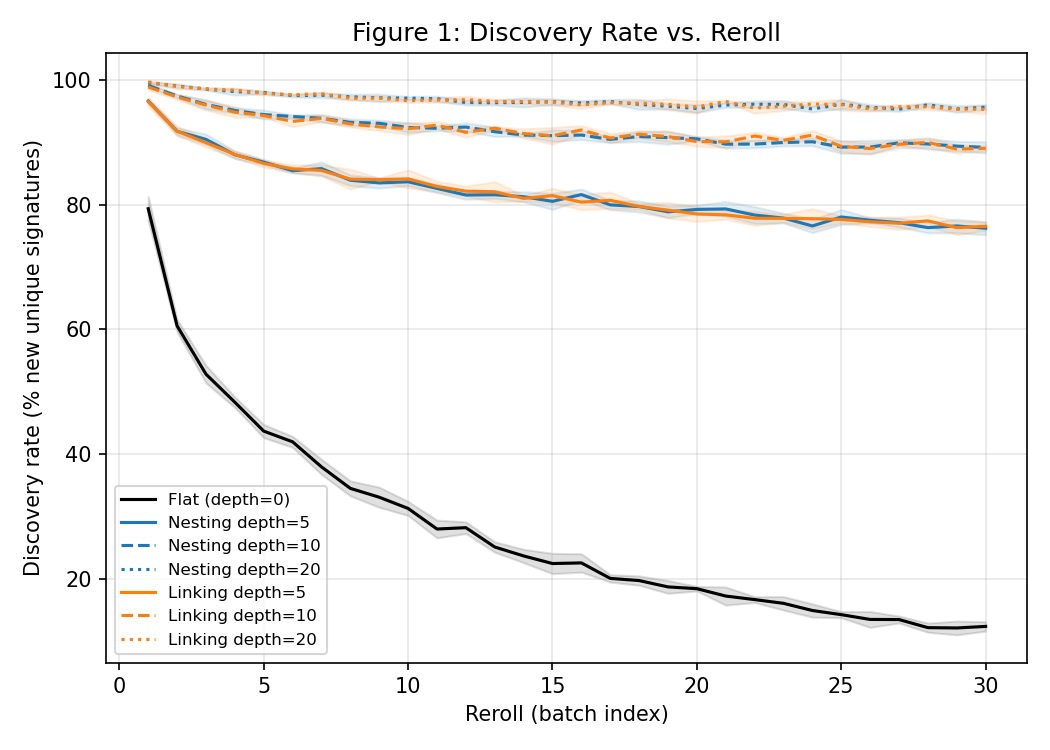
\includegraphics[width=1\linewidth]{figures/figure1_discovery_rate.png}
            \captionof{figure}{Discovery rate (mean $\pm$ std band across 5 seed-anchors) vs. reroll index, for the flat baseline and three depths each of nesting and linking. The flat shape decays sharply and continuously; every compositional shape sustains a far higher, more slowly-decaying discovery rate, with the gap widening as depth increases.}
            \label{fig:discovery-rate}
        \end{center}

        \begin{center}
            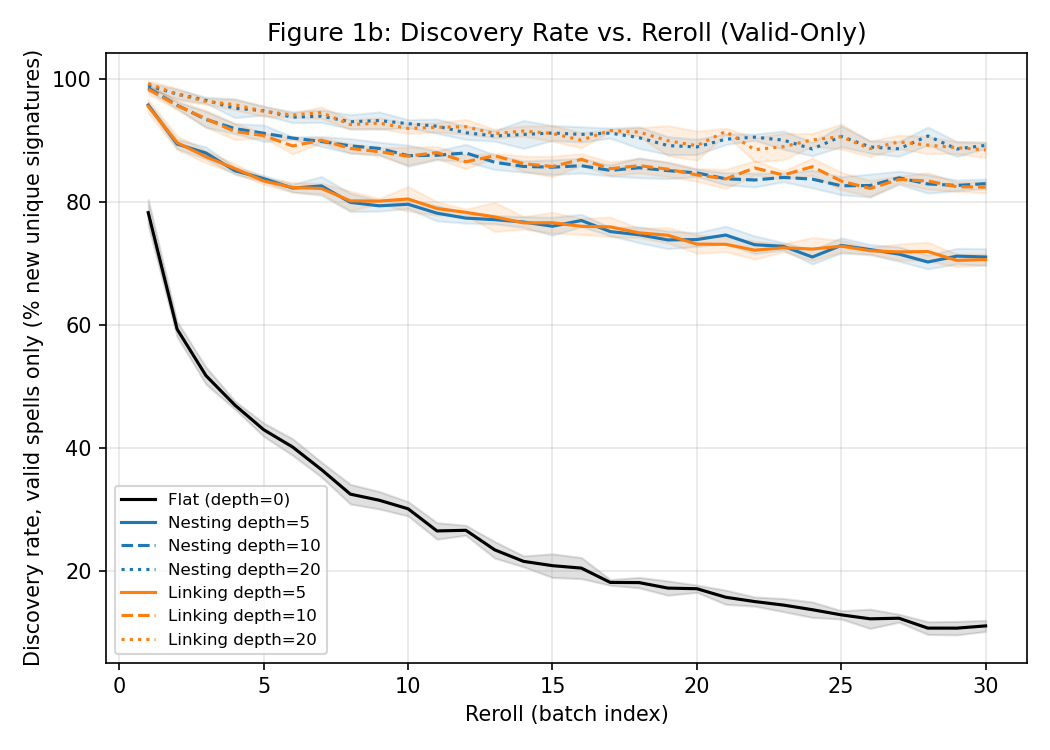
\includegraphics[width=1\linewidth]{figures/figure1b_discovery_rate_valid_only.png}
            \captionof{figure}{The same discovery-rate sequences as Figure 1, recomputed under the validity-gated metric (Section \ref{metrics}). The overall shape is unchanged: the flat baseline still collapses quickly and every compositional shape still sustains a far higher rate, but each compositional curve sits visibly lower than its Figure 1 counterpart, most noticeably at higher depth, reflecting the 6-7 point gap quantified in the tables below.}
            \label{fig:discovery-rate-valid}
        \end{center}

        \begin{table*}[]
            \centering
            \begin{tabularx}{\linewidth}{C C C C C C C}
                \hline
                Shape & First-run discovery rate (all) & First-run (valid-only) & Run-30 discovery rate (all) & Run-30 (valid-only) & Absolute drop (all) & Absolute drop (valid-only) \\
                \hline
                Flat (depth 0) & 79.4\% $\pm$ 1.9 & 78.24\% $\pm$ 2.11 & 12.4\% $\pm$ 0.8 & 11.14\% $\pm$ 0.91 & 67.0 pts & 67.10 pts \\
                Nesting = 5 & 96.6\% $\pm$ 0.4 & 95.71\% $\pm$ 0.42 & 76.2\% $\pm$ 1.1 & 71.04\% $\pm$ 1.36 & 20.4 pts & 24.67 pts \\
                Nesting = 10 & 99.1\% $\pm$ 0.3 & 98.47\% $\pm$ 0.49 & 89.2\% $\pm$ 0.9 & 82.94\% $\pm$ 0.77 & 9.9 pts & 15.53 pts \\
                Nesting = 20 & 99.6\% $\pm$ 0.2 & 98.87\% $\pm$ 0.44 & 95.7\% $\pm$ 0.4 & 89.16\% $\pm$ 0.50 & 3.9 pts & 9.71 pts \\
                Linking = 5 & 96.5\% $\pm$ 0.8 & 95.50\% $\pm$ 1.10 & 76.5\% $\pm$ 0.7 & 70.62\% $\pm$ 0.91 & 20.0 pts & 24.88 pts \\
                Linking = 10 & 98.9\% $\pm$ 0.5 & 98.29\% $\pm$ 0.80 & 89.0\% $\pm$ 0.4 & 82.38\% $\pm$ 0.92 & 9.9 pts & 15.91 pts \\
                Linking = 20 & 99.7\% $\pm$ 0.2 & 99.20\% $\pm$ 0.46 & 95.3\% $\pm$ 0.7 & 88.42\% $\pm$ 1.24 & 4.4 pts & 10.78 pts \\
                \hline
            \end{tabularx}
            \captionof{table}{Discovery Rate Across Repeated Re-Rolls}
            \label{tab:discovery-rate}
        \end{table*}

        The flat baseline's discovery rate collapses by 67.0 percentage points over 30 re-rolls (an 84\% relative decline), while every compositional shape drops by 20.4 points or less over the same span; at depth 20, the drop is under 4 points regardless of operator. By run 30, the gap between the flat baseline and any compositional shape is \textbf{64-83 percentage points}, and that gap widens (not narrows) with depth, directly contradicting any expectation that compositional shapes would \textit{catch up} to the flat grammar's saturation within this window. Standard deviations stay tight throughout ($\leq$ 2.6 points at every measured point), indicating this is a robust, low-variance effect rather than a seed-dependent fluke.

        \textbf{Valid-only recheck: this is where the validity-gating bug (Section \ref{metrics}) mattered most.} Under the validity-gated discovery-rate metric, the flat baseline's run-30 rate is 11.14\% and the compositional shapes' run-30 rates range from 70.62\% (links = 5) to 89.16\% (nesting = 20), an absolute gap of roughly \textbf{60-78 percentage points}, narrower than the original 64-83 point figure but not qualitatively different. The gap between the all-spells and valid-only metric itself grows with depth: about 1.2 points at the flat baseline (12.38\% $\rightarrow$ 11.14\%) but 6.5-7.0 points at depth 20 (95.65\% $\rightarrow$ 89.16\% nesting; 95.32\% $\rightarrow$ 88.42\% links). The original ``sustained high discovery rate at high depth'' claim was real but modestly overstated by the bug; the corrected figures are still 60-78 percentage points above the flat baseline at run 30, so \textbf{H1 still holds under the corrected metric}, and we state this explicitly rather than treating the correction as a threat to the finding.

        \textbf{Curve fitting.} $R^2$ is not a valid basis for comparing these three candidate models: it is monotonically non-decreasing in the number of free parameters and therefore structurally favors the 3-parameter exponential model ($a·e^{(-bx)}+c$) over the 2-parameter logarithmic ($a·ln(x)+b$) and power-law ($a·x^b$) models regardless of whether the extra parameter earns its keep. We replace it with AIC and BIC, both of which penalize parameter count, and, since the original fits were performed on each shape's 5-seed \textit{mean} trajectory, discarding the per-seed variance already collected, we refit all three models independently to each of the 5 raw seed-trajectories per shape, then report the distribution of which model wins (by AIC, equivalently by BIC in every case here) across those 5 independent fits rather than a single fit on the mean curve as shown in table \ref{tab:curve-fitting}

        \begin{table*}[]
            \centering
            \begin{tabularx}{\linewidth}{C C C C C C C}
                \hline
                Shape & Exponential wins (of 5 seeds) & Logarithmic wins (of 5 seeds) & Power-law wins (of 5 seeds) \\
                \hline
                Flat (depth 0) & 0 & \textbf{5} & 0 \\
                Nesting = 5 & 0 & \textbf{5} & 0 \\
                Nesting = 10 & 0 & \textbf{3} & 2 \\
                Nesting = 20 & 0 & \textbf{3} & 2 \\
                Linking = 5 & 0 & \textbf{4} & 1 \\
                Linking = 10 & 0 & \textbf{4} & 1 \\
                Linking = 20 & 2 & \textbf{3} & 0 \\
                \hline
            \end{tabularx}
            \captionof{table}{Curve fitting}
            \label{tab:curve-fitting}
        \end{table*}

        Once parameter count is penalized, the logarithmic model wins a majority of per-seed fits in every one of the 7 shapes, including nesting = 20, which, under the uncorrected $R^2$-on-means comparison, had appeared to favor the exponential model ($R^2$ = 0.954 vs. 0.950 for logarithmic, a margin $R^2$ cannot recognize as too small to justify the exponential's extra parameter). The power-law model is competitive with the logarithmic model at a few depths (splitting the per-seed vote 3-2 or 4-1) but never wins outright, and the exponential model wins only 2 of 35 total per-seed fits across all shapes, both at the single deepest linking shape. \textbf{Discovery rate is therefore best explained by a logarithmic decay model across the tested depth range}, now on a per-seed, complexity-penalized basis rather than a single fit to averaged data: a real, quantified result rather than a qualitative impression, and a more conservative one than the original $R^2$-on-means comparison suggested. This is a meaningfully different shape than a sharp exponential cutoff: logarithmic decay implies discovery rate keeps falling indefinitely, just at a continuously slowing rate, rather than converging to a stable floor.

        \textbf{Valid-only recheck of the curve-fit winners.} Refitting the same three models to each shape's 5 valid-only seed-trajectories gives results as we can see in table \ref{tab:valid-curve-fitting}

        \begin{table*}[]
            \centering
            \begin{tabularx}{\linewidth}{C C C}
                \hline
                Shape & All-spells: Exp / Log / Power wins (of 5) & Valid-only: Exp / Log / Power wins (of 5) \\
                \hline
                Nesting = 0  & 0 / 5 / 0 & 0 / 5 / 0 \\
                Nesting = 5  & 0 / 5 / 0 & 0 / 5 / 0 \\
                Nesting = 10 & 0 / 3 / 2 & 0 / 3 / 2 \\
                Nesting = 20 & 0 / 3 / 2 & 2 / 1 / 2 \\
                Linking = 5  & 0 / 4 / 1 & 0 / 5 / 0 \\
                Linking = 10 & 0 / 4 / 1 & 0 / 4 / 1 \\
                Linking = 20 & 2 / 3 / 0 & 2 / 2 / 1 \\
                \hline
            \end{tabularx}
            \captionof{table}{Valid-only recheck of the curve-fit winners}
            \label{tab:valid-curve-fitting}
        \end{table*}
        
        Logarithmic remains the majority or tied winner in 6 of the 7 shapes under valid-only refitting, the same conclusion as the original metric. The one exception is nesting = 20, where the split shifts from 3/2 log/power to a 2/1/2 three-way split across exponential, logarithmic, and power-law. We attribute this to noisier per-batch valid-spell counts at high depth: at nesting = 20 only about 36\% of generated spells are valid (Section \ref{results-depth}), so the valid-only discovery-rate denominator per batch is a small, more volatile subsample, which is a plausible source of the extra fit noise rather than evidence of a genuinely different underlying decay shape. We report this shift honestly rather than smoothing over it: the qualitative conclusion, that logarithmic decay is the best-supported model once parameter count is penalized, is not overturned, but is somewhat less clean at the single highest-depth nesting shape under valid-only data.
        
        Separately, fitting the same three models to \textbf{uniqueness ratio vs. amount of spells} (Section \ref{results-amount}'s data, dense 19-point sweep). (Shown in table \ref{tab:uniqueness-to-amount})

        \begin{table*}[]
            \centering
            \begin{tabularx}{\linewidth}{C C C C C}
                \hline
                Shape & $R^2$ (Exponential) & $R^2$ (Logarithmic) & $R^2$ (Power-law) & Best fit \\
                \hline
                Flat & \textbf{0.964} & 0.939 & 0.812 & Exponential \\
                Nesting & \textbf{0.975} & 0.869 & 0.829 & Exponential \\
                Linking & \textbf{0.965} & 0.896 & 0.859 & Exponential \\
                \hline
            \end{tabularx}
            \captionof{table}{uniqueness ratio vs. amount of spells}
            \label{tab:uniqueness-to-amount}
        \end{table*}
        
        \textbf{Exponential decay is the best fit for all three shapes}, with a clear margin over logarithmic and power-law in every case: the opposite conclusion from the discovery-rate result above. This distinguishes the two saturation phenomena: within-run uniqueness loss (driven by sampling more from a fixed space) follows a classic exponential-approach-to-asymptote curve, while cross-run discovery loss (driven by an accumulating exclusion set) follows a slower, logarithmic curve, at least within the 30-run window tested here.

        \subsection{Statistical Significance}\label{statistical-significance}

        To confirm the validity differences reported in Section \ref{results-depth} are not attributable to seed-to-seed noise, we report 95\% confidence intervals (from the n = 5 seed samples, via the t-distribution) and Cohen's d standardized effect sizes comparing the flat baseline against nesting and against linking, at three representative depths. We deliberately do not report the two-sample t-tests used in an earlier draft of this section: with non-overlapping 95\% CIs already shown at every depth, a t-test's p-value adds no information the CIs don't already convey, and because seed count (n = 5) is a parameter we chose rather than a fixed property of the system, the resulting p-values (which reached as low as $2.6\times10^{-12}$) could be driven arbitrarily lower simply by running more seeds, making them a poor, researcher-manipulable substitute for reporting the actual magnitude of the effect. Cohen's d is not subject to that failure mode, since it is a standardized mean difference rather than a function of sample size as shownin table \ref{statistical-significance}

        \begin{table*}[]
            \centering
            \begin{tabularx}{\linewidth}{C C C C C C}
                \hline
                Depth & Flat validity (95\% CI) & Nesting validity (95\% CI) & Linking validity (95\% CI) & Flat vs. Nesting (Cohen's d) & Flat vs. Linking (Cohen's d) \\
                \hline
                5  & [87.31, 88.49] & [70.38, 73.55] & [70.02, 73.21] & 16.5 & 16.8 \\
                10 & [87.31, 88.49] & [54.74, 57.26] & [54.28, 60.78] & 38.0 & 14.6 \\
                20 & [87.31, 88.49] & [34.48, 37.72] & [34.83, 37.60] & 47.5 & 54.2 \\
                \hline
            \end{tabularx}
            \captionof{table}{Linking, Nesting and Flat validity and Cohen's d}
            \label{tab:statistical-significance}
        \end{table*}
        
        Every comparison has non-overlapping 95\% confidence intervals at every tested depth, and every Cohen's $d$ is far beyond the conventional ``large effect'' threshold of 0.8, by one to two orders of magnitude in every case. The validity drop from depth 0 to any tested depth, for either operator, is a robust, large-magnitude effect rather than an artifact of the specific 5 seeds sampled, consistent with the low standard deviations already reported in Section \ref{results-depth} ($\leq$ 2.6 points at every depth). We note the low within-group variance that produces these very large d values is itself expected given Section \ref{results-depth}'s H2 analysis: since validity is close to a deterministic function of the achieved per-spell depth distribution (which is itself a fixed, seed-independent draw process at a given ceiling, Section \ref{results-depth}), seed-to-seed variance in aggregate validity is small by construction, and Cohen's d should be read here as confirming the effect is large \textit{relative to that already-small noise floor}, not as a claim that this particular d magnitude generalizes to noisier measurement settings.

        \subsection{Ablation: Flat vs. Nesting-Only vs. Linking-Only}\label{ablation}

        Spellbox's generator enforces per-spell mutual exclusivity between nesting and linking (a spell only draws a nonzero link count when its nesting count is zero): a single spell is nested \textit{or} linked, never both. This means the natural reviewer request for a 2×2 ``Nesting × Linking'' ablation (including a combined ``Both'' condition) is not representable in the current grammar as built. We chose to report the three configurations the grammar actually supports rather than relax this constraint mid-study: every other result in this paper (Sections \ref{results-amount}-\ref{statistical-significance}, \ref{hypothesis-verdicts}, \ref{generality-check-constraint-aware}-\ref{complexity-distribution}) was generated against the mutually-exclusive grammar, and changing the enforcing rule to permit combined nesting+linking would (a) change the definition of ``depth'' itself for a combined spell (is depth the nesting count, the link count, or some joint measure?), (b) require re-deriving the Section \ref{nominal-effective-search-space} per-node equivalence-class count and combinatorial space formula, since a combined node's signature contribution is not yet defined, and (c) invalidate the apples-to-apples comparison this table is making between the two operators in isolation, which is the ablation's actual purpose. A ``Both'' condition is a genuine open question for a follow-up study built around a grammar revision, not a one-line patch to bolt onto this one without redoing the surrounding analysis (shown in table \textit{ref})

        \begin{table*}[]
            \centering
            \begin{tabularx}{\linewidth}{C C C C}
                \hline
                Configuration & Validity \% & Uniqueness Ratio & Final Discovery Rate (run 30) \\
                \hline
                Flat (depth 0) & 87.9 & 0.778 & 12.4\% \\
                Nesting-only (depth 5) & 72.0 & 0.958 & 76.2\% \\
                Linking-only (depth 5) & 71.6 & 0.969 & 76.6\% \\
                Nesting-only (depth 10) & 56.0 & 0.990 & 89.2\% \\
                Linking-only (depth 10) & 57.5 & 0.989 & 89.1\% \\
                Nesting-only (depth 20) & 36.1 & 0.997 & 95.7\% \\
                Linking-only (depth 20) & 36.2 & 0.997 & 95.3\% \\
                \hline
            \end{tabularx}
            \captionof{table}{Ablation: Flat vs. Nesting-Only vs. Linking-Only}
            \label{tab:ablation}
        \end{table*}
        
        At every matched depth, nesting-only and linking-only produce nearly identical validity, uniqueness, and discovery-rate outcomes (within 1.5 points of each other): the two operators are functionally interchangeable on these three metrics at matched depth, and both are decisively better than flat on uniqueness and discovery rate while paying a shared validity cost. The absence of a ``Both'' condition is itself informative: it means this grammar cannot test whether combining nesting and linking compounds their (near-identical) individual effects, and any future extension of Spellbox that relaxes this mutual-exclusivity constraint would let that combined condition finally be measured.
        
        \textbf{Valid-only recheck.} Adding the validity-gated uniqueness ratio and discovery rate (Section \ref{metrics}) to the same configurations as shown in table \textit{ref}

        \begin{table*}[]
            \centering
            \begin{tabularx}{\linewidth}{C C C C}
                \hline
                Configuration & Validity \% & Uniqueness (valid-only) & Discovery final (valid-only) \\
                \hline
                Flat (depth 0) & 87.9 & 0.7659 & 11.1\% \\
                Nesting-only (depth 5) & 72.0 & 0.9463 & 71.0\% \\
                Linking-only (depth 5) & 71.6 & 0.9611 & 70.6\% \\
                Nesting-only (depth 10) & 56.0 & 0.9833 & 82.9\% \\
                Linking-only (depth 10) & 57.5 & 0.9828 & 82.4\% \\
                Nesting-only (depth 20) & 36.1 & 0.9920 & 89.2\% \\
                Linking-only (depth 20) & 36.2 & 0.9922 & 88.4\% \\
                \hline
            \end{tabularx}
            \captionof{table}{Ablation Valid Only}
            \label{tab:valid-ablation}
        \end{table*}
        
        Nesting and linking remain functionally interchangeable under the corrected metric too, within about 0.6 points of each other at every depth on both uniqueness and discovery rate. This section's conclusion, that the two operators are interchangeable on these metrics at matched depth, is unaffected by the validity-gating correction.

        \subsection{Hypothesis Verdicts}\label{hypothesis-verdicts}

        \textbf{H1: Supported, and unchanged under the validity-gated metric.} The discovery-rate results (Section \ref{results-discovery-rate}) directly and robustly support H1: every compositional shape sustains a discovery rate 64-83 percentage points above the flat baseline by run 30, with low variance (std $\leq$ 2.6 pts) across 5 independent seed-sequences. The effect strengthens with depth rather than being a fixed offset (a 20.4-point gap at depth 5 shrinks to under 4 points of \textit{decline} at depth 20, i.e., depth-20 shapes barely decay at all over 30 runs). This result independently replicates in a second, structurally unrelated grammar (Section \ref{generality-check-second-grammar}): its flat baseline collapses from 8\% to 0\% discovery rate within 2 re-rolls, while its compositional shapes sustain 70-100\% discovery rate through all 30 runs, an even starker version of the same pattern. Under the validity-gated discovery-rate metric introduced to correct the bug described in Section \ref{metrics}, the gap at run 30 narrows somewhat (to roughly 60-78 percentage points) but remains large and in the same direction; we state plainly that \textbf{H1's verdict does not change} under the correction.

        \textbf{H2: Supported for Spellbox; partially supported in the generality check; also unchanged under the validity-gated metric.} Within Spellbox, H2 is cleanly supported for both operators: validity falls 70-71\% (relative) while raw score rises 22-28× across the same depth range, for both nesting and linking independently (Section \ref{results-depth}). H2's evidence base (validity and uniqueness ratio) is essentially untouched by the Section \ref{metrics} correction, since the corrected uniqueness ratio moves by at most $\approx$1.2 points at any depth (Section \ref{results-depth}) and validity itself was never subject to the bug (validity is not a signature-uniqueness computation). \textbf{H2's verdict is unchanged.} However, the second-grammar generality check (Section \ref{generality-check-second-grammar}) found H2 replicates cleanly only for that grammar's **nesting-equivalent operator** (refinement: validity 89.5\% $\to$ 52.6\%, raw score 2.50 $\to$ 71.50 across depths 0-12); its \textbf{linking-equivalent operator} (chaining) showed complexity rising as expected but validity remaining pinned at 100\% across all tested depths, because that grammar's chain-adjacency rule was implemented only as a soft warning, not a hard validity error. We report this honestly rather than adjusting the second grammar's rules post hoc to force agreement: it suggests H2's validity-cost mechanism is not an automatic consequence of ``more compositional depth'' in general, but depends on whether a grammar's specific validity rules are actually sensitive to that operator's structural growth. In Spellbox, both nesting and linking are wired into the composition-symbol and sign-count checks that drive validity loss (Section \ref{generality-check-constraint-aware}); a linking-equivalent operator is not guaranteed to inherit that sensitivity in every grammar design.

        \subsection{Generality Check: An Independent Second Grammar}\label{generality-check-second-grammar}

        To test whether H1/H2 are artifacts of Spellbox's specific rule set, we built ``Rune-Chain,'' a structurally unrelated toy grammar: primitives are 5 reagents (Ash, Brine, Verdant, Mercuric, Umbral) drawn with a raw/distilled catalyst flag, composed via \textbf{refinement} (nesting-equivalent: wraps a recipe in an outer shell, compounding potency, weighted 4.5 raw-score points per level) and \textbf{chaining} (linking-equivalent: sequences independent recipes side by side, weighted 1.5 points per link beyond the first). Validity is governed by an independent ``binding rule'' (adjacent reagents can be volatile together unless tamed by a distilled catalyst), implemented separately from Spellbox's own compatibility rules so the two grammars share no validity logic.

        \begin{table*}[]
            \centering
            \begin{tabularx}{\linewidth}{C C C C}
                \hline
                Refinement depth & Validity \% & Uniqueness \% & Raw Score \\
                \hline
                0  & 89.5 & 8.3   & 2.50  \\
                2  & 85.6 & 94.2  & 13.99 \\
                4  & 77.6 & 99.9  & 25.49 \\
                6  & 71.2 & 100.0 & 36.99 \\
                8  & 64.0 & 100.0 & 48.49 \\
                12 & 52.6 & 100.0 & 71.50 \\
                \hline
            \end{tabularx}
            \captionof{table}{Generality Check: An Independent Second Grammar Analysis}
            \label{tab:second-grammar-analysis}
        \end{table*}
        
        Discovery-rate sequences (30 re-rolls, 5 seed-anchors) show the flat baseline (refinement = 0) collapsing from 8\% to 0\% discovery rate by run 2 and staying there, while refinement depths of 4 and 8 sustain 97-100\% discovery rate through all 30 runs, never meaningfully saturating within this budget. Chaining depth 2 collapses faster than refinement depth 2 (58\% $\to$ 0\% by run 5), an asymmetry worth further study, while chaining depth 4 decays slowly (99\% $\to$ 70\%) and chaining depth 8 stays at 100\% throughout. As detailed in Section \ref{hypothesis-verdicts}, this grammar cleanly replicates H1 in full, and replicates H2 for refinement but not for chaining, due to a validity rule design choice (chain-adjacency violations are warnings, not errors) rather than a property of compositional linking itself.
        
        \begin{center}
            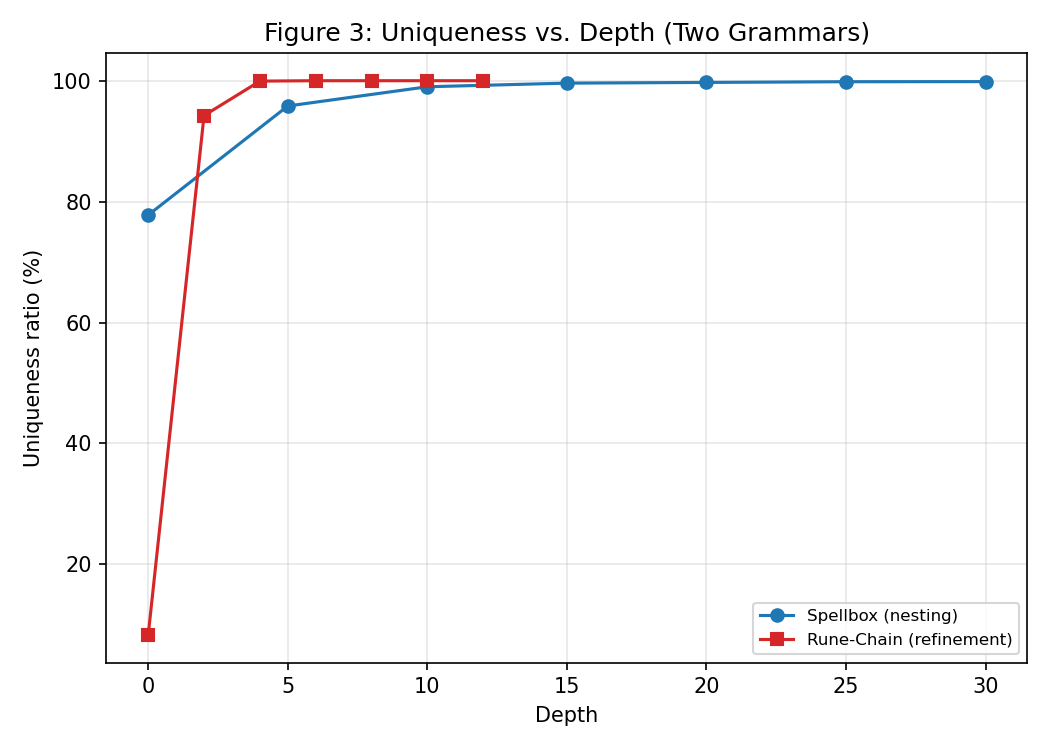
\includegraphics[width=1\linewidth]{figures/figure3_uniqueness_two_grammars.png}
            \captionof{figure}{Uniqueness ratio vs. depth for Spellbox's nesting operator and Rune-Chain's refinement operator. Rune-Chain saturates to near 100\% uniqueness by depth 4, faster than Spellbox's more gradual approach to the same ceiling; both grammars converge to a maximally-unique regime at high depth, but at different rates, consistent with Rune-Chain's smaller flat-baseline solution space (8\% uniqueness at depth 0 vs. Spellbox's 78\%).}
            \label{fig:uniqueness-ratio-depth}
        \end{center}

        \begin{center}
            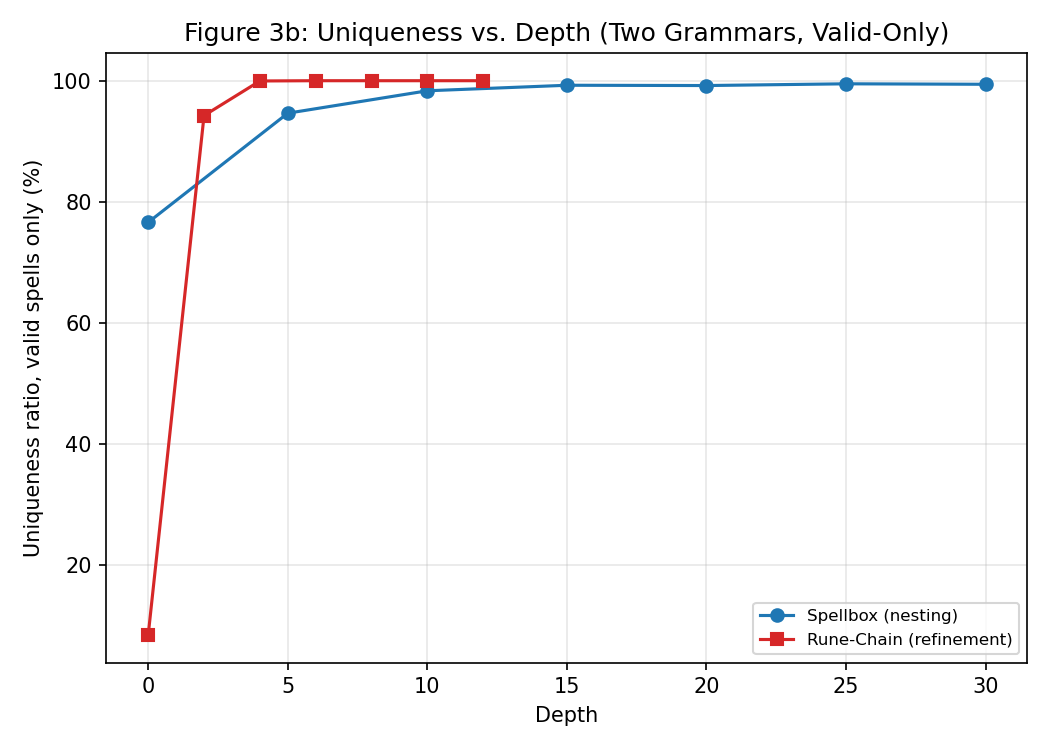
\includegraphics[width=1\linewidth]{figures/figure3b_uniqueness_two_grammars_valid_only.png}
            \captionof{figure}{The same comparison recomputed under the validity-gated uniqueness metric (Section \ref{metrics}). The two curves are visually indistinguishable from Figure 3: chaining's validity is pinned near 100\% by design (see below), so its valid-only curve is identical to its all-spells curve, and refinement's curve shifts by less than a point at any depth. This is the expected outcome, not a null result: it is a clean internal-consistency check that the validity-gating fix behaves correctly and introduces no spurious change where none is expected.}
            \label{fig:uniqueness-ratio-depth-valid}
        \end{center}
        
        \textbf{Valid-only recheck.} Applying the validity-gated metrics from Section \ref{metrics} to Rune-Chain gives an internal-consistency check that was expected in advance: chaining's validity is pinned at essentially 100\% across all tested depths, because chain-adjacency violations in this grammar are implemented as warnings rather than hard validity errors (Section \ref{hypothesis-verdicts}). Accordingly, chaining's valid-only uniqueness and discovery-rate numbers are \textbf{identical to its all-spells numbers} to within noise (e.g., discovery rate at chaining = 4, run 30: 69.5\% both all-spells and valid-only). Refinement, which does carry real validity loss (89.5\% at depth 0 down to 52.6\% at depth 12), shows the same pattern already established for Spellbox: negligible movement between the all-spells and valid-only figures (uniqueness at refinement = 0: 8.3\% all-spells vs. 8.4\% valid-only; at refinement = 4: 99.9\% vs. 100.0\%), because refinement's validity stays fairly high across the tested range. This is reassuring evidence that the validity-gating fix is implemented correctly, since it produces exactly the ``no effect where none is expected'' result the chaining operator's design predicts, rather than an arbitrary shift attributable to some other change.

        \subsection{Generality Check: A Constraint-Aware Generator}\label{generality-check-constraint-aware}

        To determine whether validity loss under depth (Section \ref{results-depth}) is an intrinsic cost of compositional structure or an artifact of one specific, fixable design decision, we built a constraint-aware generator variant that changes exactly one thing: when constructing a Radial composition symbol (a composition drawing two sigils), the second sigil is sampled only from sigils compatible with the first (per the existing compatibility table), falling back to uniform-random choice only for ``Light'', which has no compatible partner. Everything else (sign counts, nesting/linking recursion, reversed-sign probability, symbol-option selection) is unchanged.

        \begin{table*}[]
            \centering
            \begin{tabularx}{\linewidth}{C C C C}
                \hline
                Depth & Baseline Validity \% & Constraint-Aware Validity \% & Absolute Gain \\
                \hline
                0  & 87.90 & 93.63 & +5.7 pts  \\
                10 & 56.00 & 71.95 & +15.95 pts \\
                20 & 36.10 & 55.02 & +18.9 pts \\
                30 & 25.70 & 43.38 & +17.7 pts \\
                \hline
            \end{tabularx}
            \captionof{table}{Generality Check: An Independent Second Grammar Analysis}
            \label{tab:generality-check-second-grammar}
        \end{table*}

        The absolute validity gain grows with depth (more Radial-composition draws per spell means more opportunities for the one-line fix to matter), recovering \textbf{17.7-18.9 percentage points of validity at high depth} from a single, narrowly-targeted change. Critically, \textbf{uniqueness ratio and discovery rate are essentially unchanged} between generators (e.g., at nesting depth 20: uniqueness 0.997 baseline vs. 0.996 constraint-aware; final discovery rate 95.6\% vs. 95.60\%, well under a 1-point difference). This confirms composition-symbol incompatibility, not the nesting/linking structure itself, is the dominant driver of Spellbox's validity loss under depth: biasing one random decision toward known-compatible outcomes recovers a large fraction of otherwise-invalid spells without touching the size or novelty dynamics of the reachable spell space at all.

        \textbf{Valid-only recheck reveals a new finding invisible to the original metric.} Applying the validity-gated discovery-rate metric (Section \ref{metrics}) to this same generator comparison shows that ``essentially unchanged'' is true under the all-spells metric but not under valid-only: at nesting depth 20, constraint-aware's valid-only discovery rate (92.27\%) pulls measurably ahead of baseline's (89.16\%), a \textbf{3.1-point gap} that the original all-spells comparison (95.60\% vs. 95.65\%, under 1 point apart) could not detect. The same pattern holds at depth 10 (85.59\% constraint-aware vs. 82.94\% baseline, valid-only) though it is smaller in absolute terms. The mechanism is straightforward: constraint-aware has fewer invalid spells ``crowding out'' the valid-only denominator, so a larger share of its valid spells are newly-seen valid signatures in each batch. We report this as a genuinely new, secondary finding rather than a correction to the existing claim: the constraint-aware fix's primary, already-reported benefit is its direct validity gain (Section \ref{generality-check-constraint-aware}'s main table), but it also produces a modest, previously-undetectable improvement in valid-only discovery rate at high depth, on top of that validity gain. Uniqueness ratio itself remains essentially unchanged between generators under valid-only as well (0.9920 baseline vs. 0.9933 constraint-aware at depth 20), so this new finding is specific to discovery rate, not a broader reassessment of the generator comparison.

        \begin{center}
            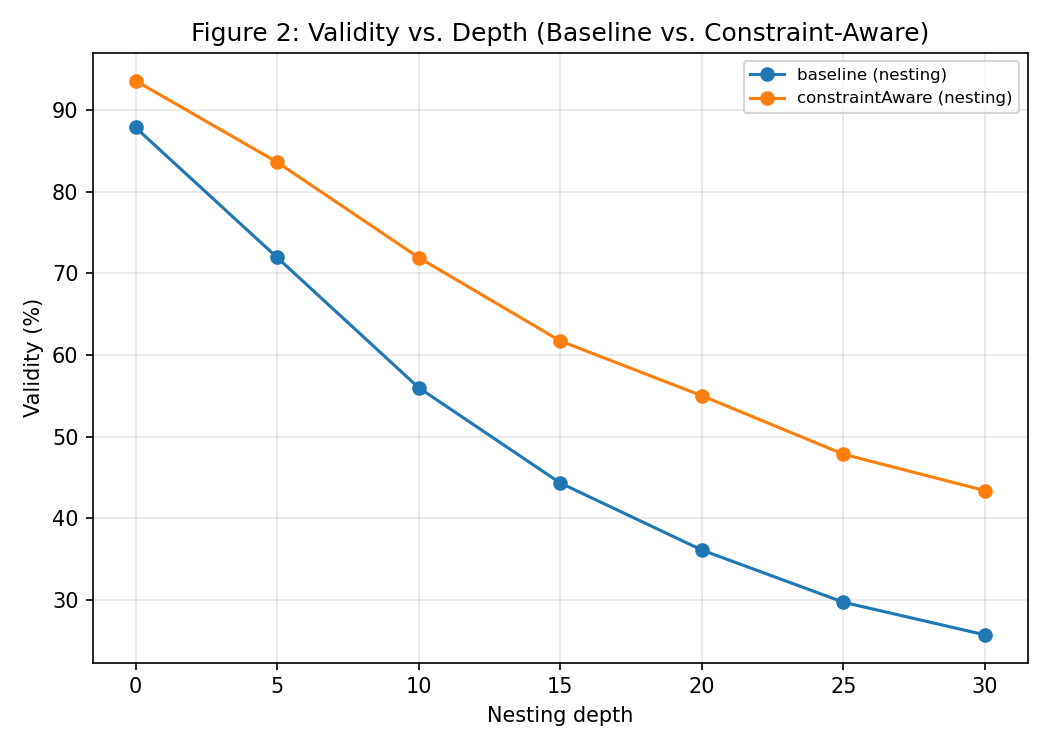
\includegraphics[width=1\linewidth]{figures/figure2_validity_baseline_vs_constraint_aware.png}
            \captionof{figure}{Validity (\%) vs. nesting depth for the baseline generator and the constraint-aware variant. The constraint-aware curve sits consistently above baseline at every depth, with the absolute gap widening from +5.7 points at depth 0 to +18.9 points at depth 20, before narrowing slightly to +17.7 points at depth 30.}
            \label{fig:validity-baseline-constraint-aware}
        \end{center}

        \subsection{Runtime Analysis: Generation Time vs. Depth}\label{runtime-analysis-time-depth}

        We instrumented the bulk generator to measure wall-clock generation time (5 repeated timing samples per depth, 1200 spells per sample) across the same depth range used in Section \ref{results-depth}, for both operators as shown in table \ref{tab:depth-nesting-linking-mean}

        \begin{table*}[]
            \centering
            \begin{tabularx}{\linewidth}{C C C C}
                \hline
                Depth & Nesting: mean time (ms) & Linking: mean time (ms) \\
                \hline
                0  & 6.6 ± 0.8  & N/A        \\
                5  & 14.4 ± 0.3 & 14.9 ± 1.5 \\
                10 & 24.4 ± 0.8 & 24.7 ± 0.6 \\
                15 & 35.1 ± 2.9 & 34.3 ± 2.3 \\
                20 & 42.7 ± 1.1 & 43.5 ± 0.8 \\
                25 & 52.3 ± 3.0 & 51.3 ± 1.9 \\
                30 & 59.4 ± 1.1 & 58.4 ± 1.0 \\
                \hline
            \end{tabularx}
            \captionof{table}{Generality Check: An Independent Second Grammar Analysis}
            \label{tab:depth-nesting-linking-mean}
        \end{table*}

        Generation time grows approximately linearly with depth for both operators (roughly 1.8 ms per depth level beyond a small fixed overhead at depth 0), and the two operators track each other closely at every depth (within 1-2 ms), consistent with both recursing the same number of times per spell (one call per nesting level or per link) with comparable per-call cost. At the depths and amounts used throughout this paper ($\leq$ 1200 spells, $\leq$ depth 30), total generation time remains under 60 ms, so runtime is not a practical constraint on any experiment reported here; it would become relevant only at substantially larger amounts or depths than tested in this study.

        \subsection{Nominal vs. Effective Search-Space Size: Quantifying Sampler Bias}\label{nominal-effective-search-space}

        \textbf{Motivation.} A first pass at this question (computing a combinatorial upper bound on the number of distinct spell signatures reachable at a given nesting depth) suggested the theoretical space grows so explosively with depth that it is effectively unlimited for any realistic sampling budget, a conclusion that, if taken at face value, makes this section's finding a nearly arithmetic consequence of exponentiation rather than a substantive empirical result. That combinatorial bound is still useful as a \textit{nominal} space size, but treating it as the relevant measure of ``how large is the space this experiment actually explores'' turns out to be the wrong question. This section instead asks: given the discovery-rate data already collected (Section \ref{results-discovery-rate}), how large is the space the sampler is \textbf{behaviorally} exploring, and how does that compare to the nominal combinatorial bound? The gap between the two, and its mechanism, is the actual result.

        \textbf{Nominal space size.} Per generation node, the grammar draws: a \textbf{central symbol} (5 sigils + 5 transformations + 15 unordered sigil-pair classes = 25 equivalence classes), and a \textbf{sign set} (one of 3 sign-option branches, each drawing 1-3 signs from independent 5-element categories with a binary reversed flag per sign; option 1: 5×2 = 10; option 2: (5×2)×(5×2 + 5×2) = 200; option 3: (5×2)×(5×2)×(5×2) = 1,000; total 1,210 sign-set classes). This gives \textbf{30,250 equivalence classes per node}, matching the exact equivalence relation used by the structural-signature function (which sorts symbol/sign multisets, so order within a node does not distinguish signatures). Compounding multiplicatively across nesting depth, since each additional level chains another independent node's choices into the same signature, gives the nominal upper bound $30,250^{(depth+1)}$ reported in the ``Nominal space'' column below.
        
        \textbf{Effective space size, via occupancy inversion.} The discovery-rate sweep (Section \ref{results-discovery-rate}) re-rolls the same generation shape 30 times per seed, tracking how many of each batch's 1200 spells are structurally new versus a repeat of a previously-seen signature. If a sampler draws uniformly from an effective space of size $N_{eff}$, the probability that a fresh draw collides with any of the $k$ previously-seen signatures is approximately $k / N_{eff}$ (an occupancy/birthday-problem approximation, valid while $k \ll N_{eff}$). We already have, for every run in every seed, both the observed repeat probability (repeats divided by total, for that batch) and the exact cumulative count of previously-seen signatures $k$ going into that batch (cumulative unique minus new count, from the prior run). Inverting the approximation gives a direct, per-run estimate of the sampler's effective space size: $N_{eff} = k / P_r$, where $P_r$ is the observed repeat probability. We compute this at each of the last 10 runs of each seed's 30-run sequence (where $k$ is largest and the estimate is most stable) and average across seeds and runs as shown in table \ref{tab:nominal-effective-space}

        \begin{table*}[]
            \centering
            \begin{tabularx}{\linewidth}{C C C C}
                \hline
                Depth & Nominal space (combinatorial upper bound) & Effective space (mean ± std, occupancy-inverted) & Gap (orders of magnitude) \\
                \hline
                0  & $3.03 \times 10^4$  & (1.06 ± 0.04) $\times 10^4$ & 0.5  \\
                5  & $7.66 \times 10^{26}$ & (1.08 ± 0.10) $\times 10^5$ & 21.9 \\
                10 & $1.94 \times 10^{52}$ & (2.63 ± 0.34) $\times 10^5$ & 43.9 \\
                20 & $1.25 \times 10^{103}$ & (6.84 ± 1.10) $\times 10^5$ & 88.3 \\
                \hline
            \end{tabularx}
            \captionof{table}{Nominal Space and Effective space}
            \label{tab:nominal-effective-space}
        \end{table*}
        
        At depth 0, nominal and effective space size agree to within a factor of $\approx$3 (0.5 orders of magnitude), exactly what uniform-sampling behavior over the full nominal space should look like, and a sanity check that the occupancy-inversion method itself is sound (the residual factor is consistent with the nominal figure being an upper bound before accounting for further signature collapsing at the sign-multiset level). The moment nesting is introduced, the two measures diverge catastrophically: by depth 20, the nominal space has grown to $1.25 \times 10^{103}$ while the effective space the sampler actually behaves as if it is drawing from has grown only to $\approx6.8 \times 10^5$, a \textbf{gap of 88 orders of magnitude}, and the gap widens (not stabilizes) as depth increases across the tested range.
        
        \textbf{Valid-only recheck.} Restricting the same occupancy-inversion procedure to valid spells only (Section \ref{metrics}) gives the data shown in table \ref{tab:nominal-effective-space-valid-only}

        \begin{table*}[]
            \centering
            \begin{tabularx}{\linewidth}{C C C C C C}
                \hline
                Depth & Nominal space & Effective space (all-spells, mean) & Effective space (valid-only, mean) & Gap, all (orders of mag.) & Gap, valid-only (orders of mag.) \\
                \hline
                0  & $3.03 \times 10^4$   & $1.06 \times 10^4$ & $0.877 \times 10^4$ & 0.5  & 0.5  \\
                5  & $7.66 \times 10^{26}$  & $1.08 \times 10^5$ & $0.602 \times 10^5$ & 21.9 & 22.1 \\
                10 & $1.94 \times 10^{52}$  & $2.63 \times 10^5$ & $0.870 \times 10^5$ & 43.9 & 44.3 \\
                20 & $1.25 \times 10^{103}$ & $6.84 \times 10^5$ & $0.966 \times 10^5$ & 88.3 & 89.1 \\
                \hline
            \end{tabularx}
            \captionof{table}{Nominal Space and Effective space for Valid Only Combinations}
            \label{tab:nominal-effective-space-valid-only}
        \end{table*}
        
        The headline, log-scale ``gap in orders of magnitude'' is barely affected by the correction (88.3 $\to$ 89.1 at depth 20), since it is a measure against an astronomically large nominal space and a factor-of-7 change in the effective-space estimate barely registers on a log scale spanning 100+ orders of magnitude. But the *absolute* effective-space estimate at depth 20 shrinks substantially once restricted to valid spells: from $6.84 \times 10^5$ to $0.966 \times 10^5$, a factor of $\approx$7 (684K $\to$ 96.6K). We read this as \textbf{strengthening, not weakening}, this section's argument: the true effective space the sampler explores, once restricted to spells that are actually valid, is even smaller than the original (all-spells) figure reported, reinforcing the claim that the sampler behaviorally explores a far smaller space than the nominal combinatorial bound suggests.
        
        \textbf{Mechanism: sampler bias from the depth-is-a-ceiling design.} This gap is explained by the same mechanism identified in Section \ref{results-depth}'s achieved-depth analysis: each spell independently draws its own nesting depth uniformly on $[0, ceiling]$ rather than every spell reaching the ceiling, so a ``depth = 20'' run's actual sample is dominated by shallow spells (mean achieved depth 9.81, not 20). The nominal-space calculation assumes every node in its count exists \textit{at} the stated depth; the sampler, in reality, spends most of its draws at much shallower depths where the per-node combinatorics have had far fewer compounding rounds to explode. Because the nominal space is a product of per-node class counts raised to the node-count power, and the achieved node count is concentrated near half the ceiling rather than at the ceiling itself, an enormous share of the nominal space's volume (everything reachable only by spells that actually draw depths in the upper half of $[0, ceiling]$) is sampled so rarely across a 30-run, 1200-spell-per-run budget that it contributes negligibly to the observed collision rate. The effective space size measured here is therefore not ``the size of the space Spellbox's grammar can produce'' but ``the size of the space this specific per-spell-uniform sampling strategy behaves as though it is drawing from'', a distinction the nominal-space number alone cannot make visible.
        
        \textbf{Reframing the result.} The contribution of this section is not ``the theoretical space is astronomically large'' (Section \ref{results-depth} and the mechanism above already establish that the depth ceiling doesn't force deep sampling, making combinatorial explosion an expected and near-arithmetic consequence). The contribution is a \textbf{general, reusable method for quantifying the gap between a compositional generator's nominal combinatorial capacity and the effective capacity a given sampling strategy actually exercises}: (1) derive the nominal space size from the grammar's equivalence-class structure, (2) use observed repeat/collision rates plus cumulative unique-signature counts to invert an effective space size via the occupancy approximation, and (3) attribute the gap to a specific, identifiable property of the sampling strategy (here, independent per-spell uniform depth draws against a fixed ceiling) rather than treating ``large nominal space'' and ``high discovery rate'' as if they were the same finding. Any PCG system with a compositional grammar and a non-exhaustive sampling strategy admits the same two measurements and the same gap-attribution exercise; a grammar whose sampler *does* force every generated item to the nominal depth would be expected to show a much smaller nominal-vs-effective gap, which would itself be a useful diagnostic for comparing sampler designs across generators (cf. Withington and Tokarchuk's and Barthet et al.'s generative-space comparison methods, Section \ref{related-work}).
        
        This also sharpens the interpretation of Section \ref{results-discovery-rate}'s discovery-rate results: a high, slowly-decaying discovery rate at nominal depth 20 is not evidence that generation is exploring a near-limitless space (the nominal-space framing), nor is it merely ``the space is so large no budget could exhaust it''; it is evidence that the sampler is effectively drawing from a space of a few hundred thousand signatures (not $10^{103}$), which a 36,000-spell cumulative budget (30 runs × 1200) is still far from saturating, but which is a concrete, measurable, and much smaller quantity than the grammar's raw combinatorial capacity would suggest.

        \subsection{Complexity Distribution}\label{complexity-distribution}

        To check whether compositional depth widens the distribution of spell complexity (raw score) or merely shifts its mean, we sampled 1200 spells at depths 0, 10, and 30 for both operators and plotted the raw-score density as shown in table \ref{tab:complexity-distribution}

        \begin{table*}[]
            \centering
            \begin{tabularx}{\linewidth}{C C C C C}
                \hline
                Depth & Nesting: mean ± std & Nesting: range & Linking: mean ± std & Linking: range \\
                \hline
                0  & 4.16 ± 3.0  & $[0, \approx18]$   & 4.16 ± 3.0  & $[0, \approx18]$   \\
                10 & 38.1 ± 24.8 & $[0, \approx150]$  & 29.5 ± 17.6 & $[0, \approx110]$  \\
                30 & 120.0 ± 55.4 & $[0, \approx280]$ & 91.5 ± 43.5 & $[0, \approx215]$  \\
                \hline
            \end{tabularx}
            \captionof{table}{Complexity Distribution}
            \label{tab:complexity-distribution}
        \end{table*}
        
        The distribution does not simply translate rightward with depth: its \textbf{spread grows much faster than a pure shift would produce}: standard deviation rises from 3.0 at depth 0 to 55.4 at depth 30 for nesting (an 18.5× increase, compared to a 28.4× increase in the mean itself), and the histogram shows the depth-30 distribution is nearly flat/uniform across a wide range rather than a narrow bump displaced from the depth-0 peak. This confirms compositionality's effect on complexity is not just ``spells get bigger on average'' but ``spells become far more heterogeneous in size'': at high depth, the amount of compounding a given spell happens to receive (via its independently-drawn nesting/linking count per spell, Section \ref{generation-model}) dominates its final complexity far more than at shallow depth, where nearly every spell is close to the same small size.

    \section{Discussion}\label{discussion}

        \subsection{H1 and H2 Together}\label{h1+h2}

        H1 and H2 describe a specific tradeoff space rather than two unrelated effects: the same compositional operators that sustain a high discovery rate (H1) are, in Spellbox, the ones spending validity to do so (H2). Section \ref{results-depth}'s geometric-decay baseline shows that H2, as originally stated (``depth trades validity for complexity''), is close to a definitional consequence of two more basic facts: validity is a conjunction of independent per-node checks, and each additional unit of nominal depth adds nodes that are individually error-prone at a fixed, measured rate: a null model that predicts most of the observed decay shape once the achieved (not nominal) node count is used. The part of H2 that is \textit{not} a near-arithmetic consequence of those two facts, and is therefore the genuinely interesting result, is Section \ref{generality-check-constraint-aware}'s finding: a substantial share of the per-node error rate itself is attributable to one specific, correctable random-choice bottleneck (composition-symbol sigil pairing), not an intrinsic property of composition, and fixing it recovers up to $\approx$19 points of validity at high depth while leaving discovery-rate dynamics completely untouched. This reframes H2's practical implication: depth's validity cost in this grammar is partly a \textit{tunable generator-design} cost, not an unavoidable structural one. The second-grammar check (Section \ref{generality-check-second-grammar}) reinforces this from a different angle: its linking-equivalent operator paid no validity cost at all, because its author (by design choice, not oversight) made chain-adjacency violations a warning rather than an error. Taken together, whether a compositional operator ``costs'' validity in a given grammar depends on how tightly that grammar's validity rules are coupled to that operator's structural growth, not on compositional depth in the abstract.

        \subsection{Confound: Normalization Function \\ Choice}\label{normalization-function}

        Because the tier boundaries were originally calibrated against Exponential normalization, the same underlying raw score produces different tier labels depending on which normalization function is applied (e.g., at depth 10 in the original single-seed sweep: Master under Sigmoid, Adept under Exponential, Apprentice under Arctan, for numerically identical spells). This is a labeling artifact, not a generation-behavior difference, and all cross-row complexity comparisons in this paper are made only within a fixed normalization function (Exponential, for all multi-seed experiments) for that reason.

        \subsection{Threats to Validity}\label{validity-threats}

        \textbf{Internal Validity.} The core risk to internal validity is that observed effects are artifacts of the random generation process itself rather than genuine consequences of nesting/linking structure. We mitigate this in three ways: (1) every depth-sweep and discovery-rate result is reported as a mean ± standard deviation across 5 independent seeds (Sections \ref{results-depth}, \ref{results-discovery-rate}), with the confidence intervals and Cohen's d effect sizes in Section 3.4 confirming the flat-vs-nesting and flat-vs-linking validity gaps are far outside what seed noise could produce (non-overlapping 95\% CIs and $|d| > 14$ at every tested depth); (2) the nominal-vs-effective space-size analysis (Section \ref{nominal-effective-search-space}) shows the observed discovery-rate trends reflect a specific, measured effective space size rather than being taken on faith from the nominal combinatorial bound; (3) we now directly report that each generated spell independently draws its own nesting depth or link count up to the run's ceiling (Section \ref{generation-model}, quantified in Section \ref{results-depth}'s achieved-depth table) rather than every spell being forced to the maximum; this is no longer an unquantified threat, since Section \ref{results-depth} reports the full achieved-depth distribution at each ceiling and Section \ref{nominal-effective-search-space} traces the nominal-vs-effective space gap directly to this mechanism, but it remains a design property of the generator we did not alter for this study (Section \ref{ablation}), so ``depth = 20'' should still be read throughout as a ceiling on a distribution, not a level every spell reaches.

        \textbf{A fourth internal-validity threat, identified and corrected during this study: validity/uniqueness conflation.} We found, during this study, that the original uniqueness-ratio and discovery-rate tracking counted a spell's structural signature as ``unique'' or ``newly discovered'' without gating on that spell's validity (Section \ref{metrics}). This is an internal-validity threat because it means a metric intended to measure novelty of \textit{sound} generator output could instead be partly measuring novelty of malformed output, which is a different (and less interesting) quantity. We quantified the magnitude of this threat directly rather than assuming it away: for uniqueness ratio, the effect is small, at most $\approx$1.2 percentage points of difference at any tested depth (Section \ref{results-depth}); for discovery rate, the effect is larger and grows with depth, reaching 6-7 percentage points by run 30 at nesting/linking depth 20 (Section \ref{results-discovery-rate}), and it is large enough to require restating the abstract's headline gap figure (from 64-83 points to roughly 60-78 points, valid-only). We corrected the underlying tracking code to add a parallel, validity-gated metric alongside every original one (rather than silently replacing the original), and we report both throughout this paper so a reader can judge the magnitude of the correction directly rather than trust a single recomputed number. Both of this paper's hypotheses (H1, H2) hold under the corrected metric (Section \ref{hypothesis-verdicts}); this threat was real and is now quantified and disclosed, but it does not overturn either of the paper's core conclusions.
        
        \textbf{A fifth internal-validity consideration, addressed in this revision: a pre-existing narrative mislabeling in Section \ref{results-amount}.} Independently re-running the amount-of-spells sweep for this revision (Section \ref{revision-note}) surfaced a mislabeling in how the amount sweep's results had previously been described: figures belonging to the flat, non-compositional baseline (validity rising to 88\%, uniqueness falling to 0.12) had been attributed in prose to the linked-spell shape instead. The underlying per-row data (the full amount-sweep table) was never wrong; only the narrative summary describing it was. This has been corrected in Section \ref{results-amount} and does not affect any hypothesis verdict, since Section \ref{results-amount} is a descriptive sweep and does not itself bear on H1 or H2 (those are tested in Sections \ref{results-depth}-\ref{results-discovery-rate}); we disclose the correction here for the same reason we disclose the validity-gating bug above: a reader comparing this revision against an earlier description of the same experiment should know exactly what changed and why.
        
        \textbf{External Validity.} All quantitative findings are demonstrated on two grammars only (Spellbox and the purpose-built Rune-Chain second grammar, Section \ref{generality-check-second-grammar}), both toy, synthetic domains with small (5-primitive) vocabularies and simple pairwise validity rules. Rune-Chain was built by the same research process being evaluated, which is a weaker generality test than an independently-designed, pre-existing grammar would provide (though its H2 divergence for the chaining operator, Section \ref{hypothesis-verdicts}, is informative precisely because it was not tuned to agree with Spellbox's results). Neither grammar resembles a production-scale PCG system (e.g., full game-content generators with hundreds of primitives and cross-cutting constraints), so claims here should be read as ``this pattern is not unique to one specific rule set'' rather than ``this pattern holds for compositional PCG systems in general.'' The discovery-rate experiments are also bounded to a 30-re-roll window (Sections \ref{results-discovery-rate}, \ref{generality-check-second-grammar}); the logarithmic best-fit implies discovery rate keeps declining slowly rather than plateauing within that window, so whether the deepest compositional shapes ever saturate outside this window is untested.
        
        \textbf{Construct Validity.} This paper operationalizes ``novelty saturation'' as \textbf{discovery rate}: the fraction of each re-rolled batch that is structurally new by the structural-signature equivalence relation defined in Section \ref{metrics}. This is a proxy, not a direct measurement of the underlying concept: that signature relation collapses spells that differ only in sign order or in un-tracked structural details into the same class, so discovery rate measures saturation of the \textit{signature space}, which may be coarser or finer than what a human player would perceive as ``a new spell''. Section \ref{nominal-effective-search-space}'s effective-space-size estimate reinforces this concern from a different angle: a persistently high discovery rate is consistent both with ``the grammar is genuinely rich'' and with ``the signature equivalence relation is simply too coarse to ever register a collision at the effective space sizes measured there (on the order of $10^4-10^6$ signatures)''; this paper cannot fully distinguish those two explanations from discovery-rate data alone, and doing so would require an independent human-judgment baseline (e.g., sampling spell pairs the signature relation calls distinct and asking human raters whether they are meaningfully different) that is out of scope for this study. Because we cannot rule out the coarser-signature-relation explanation, every discovery-rate and novelty claim in this paper should be read as scoped to \textit{novelty under that signature relation}, not validated against human-perceived novelty; we state this in the abstract as well as here, rather than only here, so the paper's scope is not overstated by readers who skip Section \ref{validity-threats}. Similarly, \textbf{validity} is a binary construct (structurally sound vs. not, per the validator's error-level checks; Section \ref{metrics}) that treats all validity violations as equivalent, when in practice a single incompatible composition-symbol pair might be a materially different failure than a missing Control sign; Section \ref{generality-check-constraint-aware}'s constraint-aware intervention shows these are not evenly distributed, so ``validity \%'' is a coarser signal than the underlying failure modes it aggregates.
        
        Two further threats apply across all three categories: nesting and linking are compared at matched \textit{depth} values, not matched \textit{raw-score} values (Section \ref{results-depth}), so a depth-matched comparison is not a complexity-matched one; and the constraint-aware generator (Section \ref{generality-check-constraint-aware}) targets exactly one identified validity-loss mechanism, leaving smaller sources of invalidity unaddressed and still contributing to the residual validity gap at high depth.

        \section{Conclusion}\label{conclusion}

        This study asked how compositional operators affect novelty saturation in a constrained procedural spell grammar, and tested it with several converging lines of evidence: single-seed sweeps, 5-seed multi-seed sweeps with variance reporting, per-seed AIC/BIC-based curve fitting, an independent generator-design intervention, a fully independent second grammar, and a nominal-vs-effective search-space analysis. H1 (compositional operators delay saturation) is well-supported and replicates cleanly in an independent grammar. H2 (depth trades validity for complexity) holds cleanly in Spellbox for both operators, and in the second grammar for its nesting-equivalent operator, but a validity cost is not automatic for a linking-equivalent operator: it depends on whether that grammar's rules are actually sensitive to what linking changes structurally. A geometric-decay baseline (Section \ref{results-depth}) shows most of H2's shape is close to a definitional consequence of two more basic facts (validity as a conjunction of independent per-node checks, and depth as a per-spell ceiling rather than a level), which sharpens rather than weakens the paper's most interesting validity finding: a follow-up experiment isolating exactly one validity-loss mechanism (composition-symbol pairing) showed a large fraction of Spellbox's *residual*, non-definitional validity cost is a fixable generator-design choice, not an unavoidable tax on compositional depth itself. Separately, this paper's search-space analysis (Section \ref{nominal-effective-search-space}) contributes a general, reusable method (nominal combinatorial space size versus occupancy-inverted effective space size from observed collision rates) for quantifying how much of a compositional generator's raw capacity a given sampling strategy actually reaches; applied here, it shows Spellbox's per-spell-uniform depth sampling reaches an effective space many orders of magnitude smaller than its nominal combinatorial capacity, and traces that gap to the same depth-is-a-ceiling mechanism underlying the H2 reframing above. Taken together, the expressiveness-versus-soundness tradeoff observed here is real, but partially negotiable by grammar and sampler design rather than fixed by the choice to use composition operators at all. During this study we also found, quantified, and corrected a methodological bug in which the uniqueness-ratio and discovery-rate metrics did not gate on spell validity (Section \ref{metrics}); we consider the discovery and correction of this bug, and the transparent reporting of both the original and corrected figures throughout (Sections \ref{results-depth}, \ref{results-discovery-rate}, \ref{ablation}, \ref{generality-check-second-grammar}, \ref{generality-check-constraint-aware}, \ref{nominal-effective-search-space}, \ref{validity-threats}), part of this study's rigor rather than a mark against it, since the correction was caught before publication, its magnitude was quantified precisely, and it was shown not to overturn either H1 or H2 (Section \ref{hypothesis-verdicts}). Separately, during preparation of this revision, an independent re-execution of the amount-of-spells sweep (Section \ref{revision-note}) surfaced and corrected a narrative mislabeling in Section \ref{results-amount}'s original description, where figures belonging to the flat baseline had been attributed to the linked-spell shape; the underlying data was never wrong, only its prose description, and the correction does not affect either hypothesis verdict. All findings remain scoped to novelty and search-space size as measured under the structural-signature equivalence relation defined in Section \ref{metrics}; independently validating that relation against human judgments of "meaningfully different" spells, extending discovery-rate sequences well beyond 30 re-rolls, re-running the depth sweeps with a fixed (rather than uniformly-drawn) per-spell depth, and testing additional independently-designed grammars are the clearest directions for future work.

        \section{References}\label{references}

        \textbf{Grammar-based / rule-based PCG}

        \begin{itemize}
            \item Stiny, G., and Gips, J. ``Shape Grammars and the Generative Specification of Painting and Sculpture.'' \textit{IFIP Congress}, 1971.
            \item Prusinkiewicz, P., and Lindenmayer, A. \textit{The Algorithmic Beauty of Plants}. Springer, 1990.
            \item Müller, P., Wonka, P., Haegler, S., Ulmer, A., and Van Gool, L. ``Procedural Modeling of Buildings.'' \textit{ACM SIGGRAPH}, 2006.
            \item Dormans, J. ``Adventures in Level Design: Generating Missions and Spaces for Action Adventure Games.'' \textit{Proceedings of the 2010 Workshop on Procedural Content Generation in Games (PCGames)}, 2010.
            \item Smith, A. M., and Mateas, M. ``Variations Forever: Flexibly Generating Rulesets from a Sculptable Design Space of Mini-games.'' \textit{IEEE Conference on Computational Intelligence and Games (CIG)}, 2010.
            \item Smith, A. M., and Mateas, M. ``Answer Set Programming for Procedural Content Generation: A Design Space Approach.'' \textit{IEEE Transactions on Computational Intelligence and AI in Games (TCIAIG)}, 3(3), 2011.
            \item Shaker, N., Togelius, J., and Nelson, M. J. \textit{Procedural Content Generation in Games: A Textbook and an Overview of Current Research}. Springer, 2016.
        \end{itemize}

        \textbf{Expressive range and generator evaluation}

        \begin{itemize}
            \item Smith, G., and Whitehead, J. ``Analyzing the Expressive Range of a Level Generator.'' \textit{Proceedings of the 2010 Workshop on Procedural Content Generation in Games (PCGames)}, 2010.
            \item Horn, B., Dahlskog, S., Shaker, N., Smith, G., and Togelius, J. ``A Comparative Evaluation of Procedural Level Generators in the Mario AI Framework.'' \textit{Foundations of Digital Games (FDG)}, 2014.
            \item Smith, G. ``What Do We Value in Procedural Content Generation?'' \textit{Foundations of Digital Games (FDG)}, 2017.
            \item Summerville, A. ``Expanding Expressive Range: Evaluation Methodologies for Procedural Content Generation.'' \textit{AIIDE}, 2018.
            \item Cook, M., Colton, S., Gow, J., and Smith, G. ``General Analytical Techniques for Parameter-Based Procedural Content Generators.'' \textit{IEEE Conference on Games (CoG)}, 2019.
            \item Cook, M., Gow, J., Smith, G., and Colton, S. ``Danesh: Interactive Tools for Understanding Procedural Content Generators.'' \textit{IEEE Transactions on Games}, 14(3), 2022, pp. 329-338.
        \end{itemize}
        
        \textbf{Diversity and novelty}

        \begin{itemize}
            \item Lehman, J., and Stanley, K. O. ``Abandoning Objectives: Evolution Through the Search for Novelty Alone.'' \textit{Evolutionary Computation}, 19(2), 2011.
            \item Togelius, J., Yannakakis, G. N., Stanley, K. O., and Browne, C. ``Search-Based Procedural Content Generation: A Taxonomy and Survey.'' \textit{IEEE Transactions on Computational Intelligence and AI in Games (TCIAIG)}, 3(3), 2011.
            \item Mouret, J.-B., and Clune, J. ``Illuminating Search Spaces by Mapping Elites.'' \textit{arXiv:1504.04909}, 2015.
            \item Pugh, J. K., Soros, L. B., and Stanley, K. O. ``Quality Diversity: A New Frontier for Evolutionary Computation.'' \textit{Frontiers in Robotics and AI}, 3, 2016.
            \item Gravina, D., Khalifa, A., Liapis, A., Togelius, J., and Yannakakis, G. N. ``Procedural Content Generation through Quality Diversity.'' \textit{IEEE Conference on Games (CoG)}, 2019 (also \textit{arXiv:1907.04053}).
        \end{itemize}
        
        \textbf{Generative-space comparison}

        \begin{itemize}
            \item Withington, T., and Tokarchuk, L. ``Compressing and Comparing the Generative Spaces of Procedural Content Generators.'' \textit{arXiv:2205.15133}.
            \item Barthet, M., Liapis, A., and Yannakakis, G. N. ``Generative Shift Analysis.'' \textit{arXiv:2309.05371}.
        \end{itemize}
        
        \textbf{Statistical methodology}

        \begin{itemize}
            \item Burnham, K. P., and Anderson, D. R. \textit{Model Selection and Multimodel Inference: A Practical Information-Theoretic Approach}. 2nd ed., Springer, 2002.
        \end{itemize}
        
        \textbf{Grammar-as-rule-system framing (background)}

        \begin{itemize}
            \item Martens, C. ``Ceptre: A Language for Modeling Generative Interactive Systems.'' \textit{AIIDE}, 2015.
            \item Smith, A. M., Nelson, M. J., and Mateas, M. ``Ludocore: A Logical Game Engine for Modeling Videogames.'' \textit{IEEE Conference on Computational Intelligence and Games (CIG)}, 2010.
        \end{itemize}
            
        \textbf{If a future human-evaluation study is added (Section \ref{validity-threats})}

        \begin{itemize}
            \item Cherry, E., and Latulipe, C. ``Quantifying the Creativity Support Index.'' \textit{ACM Transactions on Computer-Human Interaction (TOCHI)}, 21(4), 2014.
            \item Compton, K., and Mateas, M. ``Casual Creators.'' \textit{International Conference on Computational Creativity (ICCC)}, 2015.
        \end{itemize}
\end{document}